%%\chapter{Revisão da literatura}
\label{Fundamentacao}
%
%	\begin{flushright}
%		\textit{``O período de maior ganho em conhecimento e experiência
%		\\ é o período mais difícil da vida''.\\Dalai Lama}
%	\end{flushright}
%
%

Neste capítulo busca-se contextualizar o leitor dos fundamentos teóricos nos quais este trabalho se baseia, mais especificamente abordando de forma mais detalhada o funcionamento da técnica DTM. Além disso, as tecnologias utilizadas na realização desta pesquisa serão apresentadas de forma teórica, permitindo ao leitor assimilar seu funcionamento e assim melhor compreender sua aplicação prática descrita no capítulo \ref{Desenvolvimento}.

Para melhor compreensão, este capítulo é dividido em três seções. Na primeira seção ocorre a demonstração de como se dá o processo de memorização dinâmica de traces. Na segunda seção é apresentado o processador LEON3 juntamente com outras tecnologias auxiliares. Por fim, na terceira seção é explicado como funciona o FPGA, tecnologia para gravação de circuitos utilizada neste trabalho.


\section{Memorização dinâmica de traces}
\label{Fundamentacao:DTM}

A memorização dinâmica de traces é uma técnica que busca evitar a perda de tempo computacional reduzindo o número de execuções de instruções já executadas. Diferente de algumas técnicas de programação que exploram o reuso em software, a DTM trabalha a nível de hardware e identifica candidatos ao reuso de forma dinâmica. Essa identificação dinâmica se caracteriza por reutilizar instruções em qualquer ponto do programa, identificando a redundância desta instrução de acordo com os valores dos seus parâmetros de entrada, comparando-os aos de uma execução anterior.


%%%%%%%%%%%%%%%%%%%%%%%%%%%%%%%%%%%%%%%%%%%%%%%%%%%%%%%%%%%%%%%%
%%%%%%%%%%%%%%%%%%%%%%%%%%%%%%%%%%%%%%%%%%%%%%%%%%%%%%%%%%%%%%%%
%%%%%%%%%%%%%%%%%%%%%%%%%%%%%%%%%%%%%%%%%%%%%%%%%%%%%%%%%%%%%%%%
%%%%%%%%%%%%%%%%%  INTRODUZIR A TECNICA DTM  %%%%%%%%%%%%%%%%%%%
%%%%%%%%%%%%%%%%%%%%%%%%%%%%%%%%%%%%%%%%%%%%%%%%%%%%%%%%%%%%%%%%
%%%%%%%%%%%%%%%%%%%%%%%%%%%%%%%%%%%%%%%%%%%%%%%%%%%%%%%%%%%%%%%%
%%%%%%%%%%%%%%%%%%%%%%%%%%%%%%%%%%%%%%%%%%%%%%%%%%%%%%%%%%%%%%%%

Na figura \ref{Fig:ExemploDTM} vemos um exemplo do funcionamento de DTM em um fluxo de controle. Na figura, cada nó representa um instrução e as ligações entre os nós representam os possíveis caminhos de execução de um código. 

Em (a) é possível observar uma sequência de intruções que foram executadas pelo programa, com os nós em cinza claro simbolizando as instruções executadas enquanto os em branco os caminhos não tomados.

Em (b) temos em cinza escuro os nós que representam instruções redundantes executadas. Após a identificação dessas instruções, ocorre a construção do trace e a memorização deste.

Em (c) é representado como o fluxo de controle se comporta quando ocorre o reuso do trace. Como pode ser notado, as instruções identificadas como redundantes não são executadas. Ocorre então a escrita dos resultados gerados na execução memorizada e o desvio para a próxima instrução a ser executada que não pertence ao trace, considerando qualquer desvio que tenha sido tomado entre as instruções reusadas.

\begin{figure}
\label{Fig:ExemploDTM}
	\caption[Exemplo das etapas do processo de DTM em um fluxo de controle]{
	\label{fig:facetasIndividuo} Exemplo do processo de DTM em um fluxo de controle: (a) Instruções executadas; (b) Instruções redundantes identificadas, memorização; (c) Fluxo de controle quando ocorre reuso do trace.}
	
	\centering
	\begin{multicols}{3}
		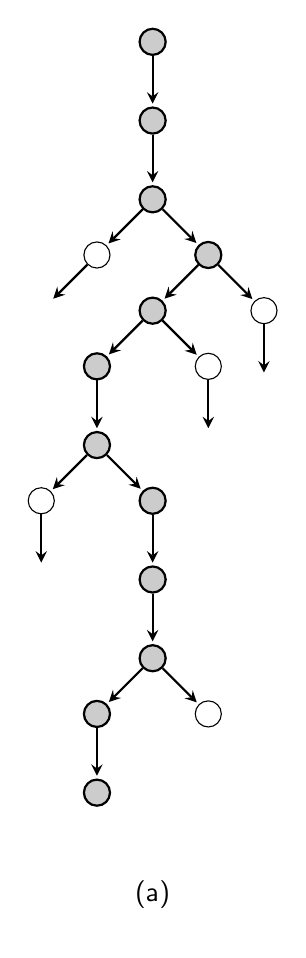
\begin{tikzpicture}[->,>=stealth,shorten >=1pt,auto,node distance=1cm,thick,main node/.style={fill=black!20,circle,draw,font=\sffamily}]
	
		\node[main node] (1) { };
		\node[main node] (2) [below of=1] { };
		\node[main node] (3) [below of=2] { };
		\node[main node, style={thin, fill=none}] (4) [below left of=3] { };
		\node[main node] (5) [below right of=3] { };
		\node[main node, style={draw=none, fill=none}] (erapraser6) [below left of=4] { };
		\node[main node] (6) [below left of=5] { };
		\node[main node, style={thin, fill=none}] (7) [below right of=5] { };
		\node[main node, style={thin, fill=none}] (8) [below right of=6] { };
		\node[main node] (9) [below left of=6] { };
		\node[main node, style={draw=none, fill=none}] (erapraser10) [below of=7] { };
		\node[main node, style={draw=none, fill=none}] (10) [below of=8] { };
		\node[main node] (11) [below of=9] { };
		\node[main node] (12) [below right of=11] { };
		\node[main node, style={thin, fill=none}] (13) [below left of=11] { };
		\node[main node] (14) [below of=12] { };
		\node[main node, style={draw=none, fill=none}] (15) [below of=13] { };
		\node[main node] (16) [below of=14] { };
		\node[main node] (17) [below left of=16] { };
		\node[main node, style={thin, fill=none}] (18) [below right of=16] { };
		\node[main node] (19) [below of=17] { };
		\node[main node, style={draw=none, fill=none}] (20) [below of=16] {};
		\node[main node, style={draw=none, fill=none}] (21) [below of=20] {};
		\node[main node, style={draw=none, fill=none}] (a) [below of=21] {(a)};
		
		\path[every node/.style={font=\sffamily\small}]
		(1) edge (2)
		(2) edge (3)
		(3) edge (4)
			edge (5)
		(4)	edge (erapraser6)
		(5) edge (6)
			edge (7)
		(6) edge (8)
			edge (9)
		(7) edge (erapraser10)
		(8) edge (10)
		(9) edge (11)
		(11)edge (12)
			edge (13)
		(12)edge (14)
		(13)edge (15)
		(14)edge (16)
		(16)edge (17)
			edge (18)
		(17)edge (19);
		
		\end{tikzpicture}
		
		%%%%%%%%%%%%%%%%%%%%%%%%%%%%%%%%%%%%%%%%%%%%%%%%%%%%%%%%%%%%%%%%%%
		

		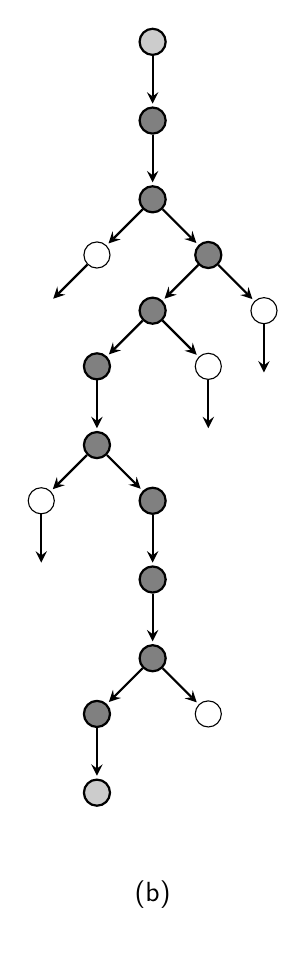
\begin{tikzpicture}[->,>=stealth,shorten >=1pt,auto,node distance=1cm,thick,main node/.style={fill=black!50,circle,draw,font=\sffamily}]
		
		\node[main node, style={fill=black!20}] (1) { };
		\node[main node] (2) [below of=1] { };
		\node[main node] (3) [below of=2] { };
		\node[main node, style={thin, fill=none}] (4) [below left of=3] { };
		\node[main node] (5) [below right of=3] { };
		\node[main node, style={draw=none, fill=none}] (erapraser6) [below left of=4] { };
		\node[main node] (6) [below left of=5] { };
		\node[main node, style={thin, fill=none}] (7) [below right of=5] { };
		\node[main node, style={thin, fill=none}] (8) [below right of=6] { };
		\node[main node] (9) [below left of=6] { };
		\node[main node, style={draw=none, fill=none}] (erapraser10) [below of=7] { };
		\node[main node, style={draw=none, fill=none}] (10) [below of=8] { };
		\node[main node] (11) [below of=9] { };
		\node[main node] (12) [below right of=11] { };
		\node[main node, style={thin, fill=none}] (13) [below left of=11] { };
		\node[main node] (14) [below of=12] { };
		\node[main node, style={draw=none, fill=none}] (15) [below of=13] { };
		\node[main node] (16) [below of=14] { };
		\node[main node] (17) [below left of=16] { };
		\node[main node, style={thin, fill=none}] (18) [below right of=16] { };
		\node[main node, style={fill=black!20}] (19) [below of=17] { };
		\node[main node, style={draw=none, fill=none}] (20) [below of=16] {};
		\node[main node, style={draw=none, fill=none}] (21) [below of=20] {};
		\node[main node, style={draw=none, fill=none}] (b) [below of=21] {(b)};
		
		\path[every node/.style={font=\sffamily\small}]
		(1) edge (2)
		(2) edge (3)
		(3) edge (4)
		edge (5)
		(4)	edge (erapraser6)
		(5) edge (6)
		edge (7)
		(6) edge (8)
		edge (9)
		(7) edge (erapraser10)
		(8) edge (10)
		(9) edge (11)
		(11)edge (12)
		edge (13)
		(12)edge (14)
		(13)edge (15)
		(14)edge (16)
		(16)edge (17)
		edge (18)
		(17)edge (19);
		
		\end{tikzpicture}
		
		%%%%%%%%%%%%%%%%%%%%%%%%%%%%%%%%%%%%%%%%%%%%%%%%%%%%%%%%%%%%%%%%%%
		
		
		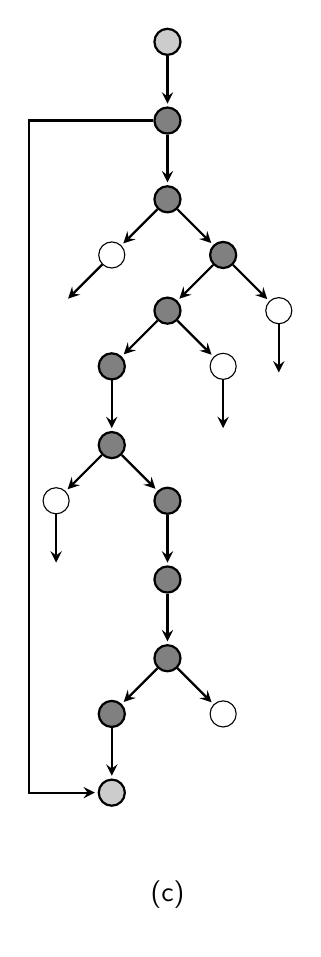
\begin{tikzpicture}[->,>=stealth,shorten >=1pt,auto,node distance=1cm,thick,main node/.style={fill=black!50,circle,draw,font=\sffamily}]
		
		\node[main node, style={fill=black!20}] (1) { };
		\node[main node] (2) [below of=1] { };
		\node[main node] (3) [below of=2] { };
		\node[main node, style={thin, fill=none}] (4) [below left of=3] { };
		\node[main node] (5) [below right of=3] { };
		\node[main node, style={draw=none, fill=none}] (erapraser6) [below left of=4] { };
		\node[main node] (6) [below left of=5] { };
		\node[main node, style={thin, fill=none}] (7) [below right of=5] { };
		\node[main node, style={thin, fill=none}] (8) [below right of=6] { };
		\node[main node] (9) [below left of=6] { };
		\node[main node, style={draw=none, fill=none}] (erapraser10) [below of=7] { };
		\node[main node, style={draw=none, fill=none}] (10) [below of=8] { };
		\node[main node] (11) [below of=9] { };
		\node[main node] (12) [below right of=11] { };
		\node[main node, style={thin, fill=none}] (13) [below left of=11] { };
		\node[main node] (14) [below of=12] { };
		\node[main node, style={draw=none, fill=none}] (15) [below of=13] { };
		\node[main node] (16) [below of=14] { };
		\node[main node] (17) [below left of=16] { };
		\node[main node, style={thin, fill=none}] (18) [below right of=16] { };
		\node[main node, style={fill=black!20}] (19) [below of=17] { };
		\node[main node, style={draw=none, fill=none}] (20) [below of=16] {};
		\node[main node, style={draw=none, fill=none}] (21) [below of=20] {};
		\node[main node, style={draw=none, fill=none}] (c) [below of=21] {(c)};
		
		\path[every node/.style={font=\sffamily\small}]
		(1) edge (2)
		(2) edge (3)
		(3) edge (4)
		edge (5)
		(4)	edge (erapraser6)
		(5) edge (6)
		edge (7)
		(6) edge (8)
		edge (9)
		(7) edge (erapraser10)
		(8) edge (10)
		(9) edge (11)
		(11)edge (12)
		edge (13)
		(12)edge (14)
		(13)edge (15)
		(14)edge (16)
		(16)edge (17)
		edge (18)
		(17)edge (19);
		
	    \draw 
	    (2.west)
	    -- ++(left:4.5em) 
	    |- (19.west);
		
		\end{tikzpicture}
	\end{multicols}

\legend{Fonte: elaborada pelo autor}
\end{figure}

\subsection{Identificação e memorização de traces}
\label{Fundamentacao:DTM:Identificacao}

\subsection{Reuso de traces}
\label{Fundamentacao:DTM:Reuso}

\subsection{DTM a nível de hardware}
\label{Fundamentacao:DTM:Hardware}


%
%%Problema
%
%O principal objetivo deste capítulo é apresentar os fundamentos históricos, teóricos e metodológicos sobre os quais esta pesquisa é executada, além de mapear os principais e mais recentes trabalhos em análise de domínio e organização da informação corporativa.
%As seções seguintes reúnem os principais e mais recentes trabalhos que versam sobre análise de domínio e organização da informação que impliquem direta ou indiretamente em processos de classificação, indexação e recuperação de informação corporativa.
%
%%O estado da arte da análise de domínio corporativo e da organização da informação visando a classificação, indexação e recuperação da informação é a principal questão deste capítulo. Além de objetivar o mapeamento dos principais e mais recentes trabalhos em análise de domínio e organização da informação, este capítulo também se propõe a comparar criticamente os métodos intelectuais e automáticos que favoreçam a classificação e indexação automatizadas de coleções corporativas, principalmente digitais.
%
%%Motivação e Justificativa
%
%%O acervo de informação, principalmente digital, tem crescido significativamente pelas facilidades de produção, compartilhamento e armazenamento. No entanto, com esse crescimento, problemas associados à classificação, indexação e recuperação de informação têm surgido, sendo particularmente mais sérios quando informação é essencial para realizar trabalho e tomar decisões, algo que acontece em diversas situações na vida, principalmente no ambiente de trabalho.
%
%%São diversas as iniciativas que tentam minimizar tais problemas, especialmente da informação digital. Porém, iniciativas são mais efetivas quando baseadas em uma organização da informação adequada e compatível com a forma pela qual ocorre a organização do conhecimento. Adicionalmente, com o ritmo acelerado da produção de informação, desafios se impõem às tarefas de classificação e indexação da informação por esforço intelectual, exigindo muitas vezes técnicas de suporte, automáticas ou semiautomáticas, para classificação e indexação com alta precisão, alto controle de erros e alto valor utilitário. Por outro lado, o próprio desenvolvimento do conhecimento humano, a evolução das áreas de conhecimento e da linguagem criam obstáculos sérios para a eficácia e eficiência destas técnicas automáticas como passar do tempo e para variados grupos de usuários.
%
%%Procedimentos metodológicos
%
%
%%Revisão da literatura
%\section{Análise de domínio}
%
%%Conceitos de AD
%
%%\textbf{Objetivo da tese é descobrir características.}
%O objetivo desta tese é a caracterização do domínio corporativo visando favorecer a atividade de recuperação da informação corporativa. Ou seja, o objetivo é a descoberta das características que o domínio corporativo possui e apresenta, implícita e explicitamente, aos membros da sua comunidade; e a exploração dessas características para o aperfeiçoamento de sistemas automáticos de recuperação de informação corporativa.
%
%%\textbf{análise de domínio. Pressuposto do domínio intangível.}
%A formalização das características do domínio é o produto de um processo denominado análise de domínio \cite{alvarenga12}, pelo qual as características tornam-se explícitas através da observação e da interpretação do domínio em seu contexto de produção e uso. Um domínio, porém, é uma comunidade discursiva imersa em uma história, uma cultura, uma janela de tempo e um espaço. Portanto, o domínio refere-se a uma entidade intangível e a análise de domínio precisa partir desse pressuposto \cite{domainAnalysis1995}.
%
%%\textbf{Análise de domínio é empreendida por módulos.}
%Para enfrentar a intangibilidade do domínio, a análise de domínio dá-se através de abordagens que criam a impressão de que o domínio seja modular, sendo que a compreensão do todo dar-se-ia pela análise e compreensão dos módulos que o compõem. Em linhas gerais, ``análise é feita com base nas informações oriundas das comunidades discursivas, a partir da sua linguagem e de suas condições culturais e históricas'' \cite[p. 182]{dias11}. Então, o processo da análise de domínio começaria pela definição da amostra ou dos exemplares do domínio que tornar-se-ão objeto de observação e análise. 
%
%%\textbf{Análise de domínio corporativo não se dá como a análise de qualquer domínio.}
%Entretanto, abordagens bem-sucedidas na análise de um domínio não devem ser consideradas em outros, como se todos os domínios fossem similares \cite{hjorland2002domain}. \citeonline{alvarenga12} explicam usando o domínio corporativo como exemplo:
%
%\begin{citacao}
%a análise de domínio compreende o levantamento e estruturação dos entes que compreendem a realidade ôntica da empresa, como ser organizacional. Normalmente o trabalho de rastreamento de entes de um domínio acadêmico ou discursivo, na ciência da informação, é feito via literatura, tendo como suporte a garantia da literatura; neste caso os focos são campos de conhecimento mais ou menos sedimentados, não sendo, entretanto o caso dos seres organizacionais. Para o exercício de suas funções relativas às áreas meio e áreas finalísticas, as empresas têm como meta a identificação e descrição dos entes que a compõem, de suas essências, acidentes e processos que deles decorrem. Nesse desafio as entidades da realidade empresarial nem sempre se encontram devidamente identificadas e caracterizadas, na literatura técnico-científica publicada, mas podem estar presentes em documentos, administrativos, políticos, legislativos, etc. \cite{alvarenga12}
%\end{citacao}
%
%%\textbf{Abordagens de análise de domínio.}
%Assim, definidos os exemplares do domínio, se deve escolher as abordagens de análise de domínio que melhor correspondem aos objetivos da análise, adequados ao domínio estudado e compatíveis com a área do conhecimento e com a área de formação dos analistas do domínio. Como exemplo, os ``processos arquivísticos podem ser vistos como verdadeiras abordagens de análise de um domínio'' \cite{alvarenga12}. Também, \citeonline{hjorland2002domain} enumera outras 11 abordagens utilizadas em diferentes áreas do conhecimento que são apropriadas para a análise de domínio. Dentre elas, algumas são de interesse para este trabalho, como métodos de classificação e construção de tesauros; métodos de indexação e recuperação de informação auxiliadas por computador; estudos bibliométricos sobre coleções de documentos corporativos; estudos de documentos e gêneros; estudos terminológicos, sobre linguagens documentárias e de discurso; e estudos sobre semântica em bancos de dados.
%
%%\textbf{Abordagens podem ser adotadas isoladamente ou conjuntamente.}
%As abordagens citadas anteriormente podem ser usadas, isoladamente ou conjuntamente, no processo de análise de domínio. Os produtos de cada abordagem citada são conhecidos pela área da Biblioteconomia e Ciência da Informação: tesauros; \textit{gazetteers}; modelos de recuperação de informação; linguagens de indexação; classificações; metadados; padrões de intercâmbio de dados e outros \cite{lykke2011domain}. Para a análise de domínio, esses são apenas subprodutos \cite{albrechtsen1993subject}. No exemplo específico do domínio corporativo, ``a análise de domínio, tal como preconizada na ciência da informação, prioritariamente se volta ao planejamento e desenvolvimento de sistemas de recuperação de informações empresariais, mas sabe-se que ela se encontra dentre os interesses de outros campos profissionais e de pesquisa'' \cite{alvarenga12}. Ou seja, o produto da análise de domínio é um modelo de alto nível que favorece o projeto de sistemas de informação e serviços de informação, além de outros produtos de interesse em outros campos.
%
%%\textbf{Valor limitado dos produtos da análise de domínio.}
%O produto principal da análise de domínio, um modelo de alto nível que também pode ser denominado como `análise de domínio' ou `uma análise de domínio', possui valor limitado pela representatividade dos exemplares usados para os estudos; profundidade pela qual o domínio foi observado; expressividade das abordagens usadas para empreender o processo de análise; e pela utilidade dos subprodutos colocados à disposição dos profissionais da informação que trabalham dentro do domínio. Portanto, a análise de domínio não produz um produto final, mas um modelo que deve ser aperfeiçoado na medida em que o domínio é descoberto, e que deve ser atualizado na medida em que o domínio se desenvolve.
%
%\subsection{Fontes para o processo de análise de domínio}
%
%%\textbf{Diversidade das fontes}
%Diversas fontes constituem matéria-prima potencial para o processo de análise de domínio, as quais incluem literatura técnica-científica do domínio, exemplares documentais, entrevistas com profissionais do domínio, dentre outras. A escolha de uma ou várias dessas fontes refletem a disponibilidade e a representatividade das fontes. Especificamente no contexto do domínio corporativo, são encontrados baixa cobertura da literatura, baixa disposição para participar de estudos que envolvam informação corporativa, alto sigilo profissional e grande variedade de produtos de informação que dificulta seu uso em análise de domínio. Os documentos e os repositórios corporativos de várias empresas parecem ser o ponto de partida mais apropriado para empreender a análise de domínio, embora ainda sejam difíceis de obter.
%
%%\textbf{Complexidade da descrição de documentos.}
%São vários os desafios de gerenciar repositórios de informação e recuperar documentos a partir desses repositórios. Um desses desafios refere-se a descrição dos documentos para subsidiar a construção de ferramentas de busca que suportem a pesquisa, a navegação, a recuperação e até mesmo a ordenação adequada de resultados \cite{broughton2006}. Tal descrição certamente depende de uma análise rigorosa do conteúdo do documento que facilite sua representação, retratando o significado, os atributos e relacionamento do documento com outros objetos \cite{brascher2008organizacao}. Deve-se descrever também aquilo que não está explicitamente presente no texto, como é o caso de conceitos e as relações mais diversas de espaço, de tempo ou de papeis \cite{alvarenga12}. Esse significado deve ser anotado utilizando-se de símbolos não necessariamente encontrados no texto. Esses símbolos permitem a representação da informação através de uma notação própria a qual pode ser chamada de metalinguagem \cite{gardin1973}, linguagem documentária \cite{talamo2001} ou simplesmente linguagem de indexação \cite{fujita04}.
%
%%\textbf{Linguagens de Indexação e estruturas para representar a informação.}
%As linguagens de indexação representam a informação por alguma estrutura que reflete os objetivos do sistema de organização de conhecimento no qual é aplicada. \citeonline{hjorland2012google} apresenta uma taxonomia de sistemas de organização de conhecimento com diferentes estruturas, como listas de termos (glossários, dicionários, \textit{gazetteers}), classificações e categorias (cabeçalhos de assunto, taxonomias, esquemas de classificação), e esquemas de categorização (listas de relacionamento, tesauros, redes semânticas e ontologias).
%
%%\textbf{Incompatibilidade semântica entre estruturas.}%usar modelo em alguns pontos. Rever como usar. Talvez eu consiga falar de modelos quando eu conceituar a análise de domínio
%Há alguma compatibilidade entre as diferentes estruturas e portanto a transformação de uma estrutura em outra é natural. Porém, não é nada trivial traduzir o significado de uma estrutura para outra, uma vez que cada sistema controlado é construído com o propósito de representar um domínio a partir das necessidades particulares de seus usuários. Buscas federadas ou integradas tornam-se então pouco eficientes, quando não se mostram impossíveis \cite{halevy2005enterprise,hjorland2012google}. Ao tentar localizar e compreender informação de múltiplos repositórios em organizações, por exemplo, \citeonline{halevy2005enterprise} afirmam que frequentemente encontram-se situações em que a informação necessária parece não ser capturada em qualquer repositório, ou é necessário um esforço significativo para compreender relações semânticas entre os repositórios e só então integrá-los. 
%
%%\textbf{Modelos semânticos são limitados.}
%Apesar da existência de métodos para agregar significado a dados e garantir a ponte semântica entre diferentes modelos de um mesmo domínio, a manutenção dos modelos e da compatibilidade semântica no tempo mostra-se ainda mais desafiadora \cite{halevy2005enterprise}. Essa incompatibilidade semântica entre sistemas de informação não parece nada simples de resolver, uma vez que há incompatibilidade até mesmo entre os modelos de indexação e as ideias, ou modelos mentais, que os usuários têm da informação. Quando os modelos dos usuários e dos indexadores não coincidem sua utilidade fica comprometida e leva o usuário inevitavelmente ao sentimento de frustração e ao abandono do sistema de informação \cite{domainAnalysis1995,solomon2002}.
%
%%\textbf{Processos da organização da informação.}
%Para a área de Biblioteconomia e Ciência da Informação, a função da organização de informação inclui processos que partem da produção, seleção e coleção de objetos informacionais, passam pelo trabalho de representação, atribuição de entidades a classes de um sistema de classificação, recuperação e acesso; e chegam ao uso e implicações do uso da informação pela sociedade \cite{solomon2002}. Porém, o escopo desta pesquisa está restrito aos processos de representação e classificação visando a recuperação de informação. Mesmo assim, há muitos outros processos importantes que vão além da recuperação de objetos relevantes. Isso reflete uma mudança de paradigma que trata do conjunto de objetos mais pertinente, ao invés de mais relevante, para suportar análises e tomada de decisão por pessoas no contexto de seu trabalho \cite{solomon2002}. Esse requisito é especialmente sério quando visto dentro dos sistemas de recuperação de informação corporativa, dado seu caráter mais pragmático.
%
%%\textbf{Representação da informação versus Representação do Conhecimento - Motivação da Análise de Domínio.}%Organizar texto para explicar melhor, ou levar essa coisa lá pra cima, junto da definição de Análise de domínio Gercina questiona organização da informação e organização do conhecimento. Pede também para rever modelo x sistema
%O primeiro processo de interesse, de representação da informação, corresponde então a um processo que envolve a descrição do suporte físico, no qual se encontra a provável informação, e de conteúdo, no qual se encontra materializada alguma informação e mobiliza algum conhecimento. O produto desse processo constitui um conjunto de atributos descritivos de um objeto informacional, podendo representar apenas o objeto informacional, apenas a informação contida no objeto, ou ambos \cite{brascher2008organizacao}. Para \citeonline{brascher2008organizacao}, a representação do domínio, diferentemente do que ocorre com a informação, reflete uma visão consensual sobre a realidade representada, dentro de um determinado contexto e sob uma determinada perspectiva. Então, para representar o domínio é necessária uma análise de domínio apropriada para compreender como os diversos atores sócio-técnicos produzem e interpretam o conteúdo.
%
%%\textbf{Classificação da informação.}
%O segundo processo de interesse, de classificação da informação, não objetiva apenas encontrar e preencher os atributos que constituirão os metadados de um documento ou conteúdo, mas empreender serviços e criar produtos que suportem o trabalho de atores sócio-técnicos na realização de tarefas, tomada de decisões e julgamentos que dependam de conhecimento e informação. Esses serviços e produtos, difíceis de implementar e atualizar, devem atender às necessidades informacionais de seus usuários não só no momento da implantação, mas também no futuro, quando novos objetos informacionais, novos usuários, novas necessidades e novos conhecimentos devem também ser mobilizados \cite{solomon2002}.
%
%%\textbf{Características locais para classificar informação.}
%Para atender a esses requisitos, alguns esquemas de classificação aplicados a propósitos específicos incluem características e são influenciadas por fatores locais, que pertencem a um domínio ou, eventualmente, parecem pertencer exclusivamente a uma comunidade interna àquele domínio. Embora essas classificações ainda possam atender seus objetivos originais, as características locais poluem a classificação e podem levá-la à inutilidade precocemente. Para \citeonline{hjorland1998classification}, pesquisas em classificação, principalmente na área de Biblioteconomia e Ciência da Informação, precisam evidenciar estratégias mais gerais para a classificação, modificando-a para contextos específicos, enquanto que outras áreas do conhecimento, como a Ciência da Computação, tendem a implementar estratégias orientadas a aplicações particulares, muitas vezes baseadas em evidências empíricas e nem sempre fundamentadas teoricamente.
%
%%\textbf{Teorias epistemológicas mobilizadas para classificar melhor a informação.}%Gercina pediu para eu relacionar isso a análise de domínio.
%\citeonline{hjorland1998classification} pressupõe que classificações não são neutras e refletem uma visão do domínio classificado, argumentando que teorias epistemológicas como o empirismo, racionalismo, historicismo e pragmatismo devem prover uma base mais segura para a classificação dos campos do conhecimento. A primeira teoria epistemológica, o empirismo, baseia-se no conhecimento a partir da observação e tenta estabelecer uma generalização através dos dados observados. A segunda, o racionalismo, se ocupa em estabelecer a busca da razão a partir do raciocínio, da lógica e da objetividade, generalizando e reduzindo a realidade a uma única estrutura de conhecimento, onde são sintetizados todos os interesses, propósitos e perspectivas. O historicismo, por sua vez, estabelece os processos históricos e culturais como causas da transformação do universo, podendo ser descritos e compreendidos com o objetivo de conhecer a realidade humana e determinar tendências. Finalmente, o pragmatismo compreende que a natureza apresenta fenômenos que podem ser reduzidos aos seus aspectos mais úteis e práticos, sendo que os demais aspectos, caso não ofereçam qualquer vantagem para os indivíduos, são desnecessários.
%
%%\textbf{A importância do contexto para a informação.}
%Especialmente para as duas últimas correntes, o historicismo e o pragmatismo, passa a ser essencial também reconhecer o contexto da informação, dos seus atores e do seu uso. No processo de análise de domínio, o contexto corresponde à configuração que os atores sócio-técnicos apresentavam no momento da produção da mensagem contida no objeto informacional e apresentam no momento da recepção da mensagem. O contexto implica nos significados que a informação assume em diferentes cenários de acesso e uso, em diferentes momentos da história, dentro de diferentes localidades, contida em diferentes suportes físicos e estruturas de documentos, para diferentes grupos sociais e por diferentes remetentes. Abordagens para a especificação do contexto, como o domínio, o ambiente de uso ou mesmo o contexto da necessidade informacional, têm figurado mais na agenda de pesquisa em classificação como fundamental para a organização do conhecimento, tendo em vista a necessidade de se implementar sistemas que adaptem a informação às tarefas e aos problemas das pessoas \cite{solomon2002}. 
%
%%\textbf{Fontes de evidência do contexto}
%Se para a análise de domínio é fundamental garantir a especificação do contexto, a análise de conteúdo dos documentos não é suficiente para representar o domínio. De fato, ``não se deve esquecer de que aos documentos devem-se agregar outras fontes, visando-se alcançar outra faceta da realidade organizacional: a que corresponde às idéias implícitas, presentes no conhecimento tácito dos membros da comunidade e que contribui para o desvelamento dessa mesma realidade'' \cite{alvarenga12}. Neste trabalho, essas outras fontes são denominadas fontes de evidência do contexto, as quais são exploradas em diferentes áreas do conhecimento e identificadas através de diferentes abordagens.
%
%%\textbf{Link para as próximas seções.}%Gercina pediu para eu explicar qual a relação entre as evidências com a Análise de Domínio
%A partir da próxima subseção são tratadas brevemente as i) evidências empíricas, ii) temporais, iii) linguísticas, iv) semânticas, v) sociais e vi) espaciais para organização e classificação da informação. Elas constituem fontes de evidência de contexto para a provável informação contida em um objeto informacional e colaboram para inserir documentos a um provável contexto, isoladamente ou em conjunto.
%
%
%%%Evidências empíricas e métodos estatísticos
%
%\subsection{Evidências empíricas}% e métodos estatísticos}
%\label{evidenciasEmpiricas}
%
%%\textbf{Empirismo na Ciência da Informação versus Ciência da Computação.}
%Principalmente na área da Ciência da Computação têm sido projetadas diversas técnicas baseadas em inteligência artificial que podem contribuir com a análise de domínio. No entanto, as técnicas computacionais parecem negligenciar a natureza social, cultural e histórica da informação \cite{hjorland2002domain}. Segundo \citeonline{hjorland2002domain}, o papel da Ciência da Computação e da Biblioteconomia e Ciência da Informação são diferentes. Enquanto a Ciência da Computação tenta capturar um modelo mais generalizado dos usuários de informação, a área de Biblioteconomia e Ciência da Informação está aberta a visões alternativas e demonstra inclusive as incertezas da informação aos usuários.
%
%%\textbf{Predominância do empirismo e seus limites.}
%Apesar dessas diferenças, em ambas as áreas muitos estudos são baseados em fenômenos puramente empíricos. Segundo \citeonline{talamo2001}, a própria atividade de classificação em Biblioteconomia e Ciência da Informação mostra-se muito empírica, com a presença de decisões arbitrárias do indexador. Um problema dos métodos empíricos é que a observação de que um certo padrão ocorre não nos permite uma generalização e o empirismo não pode garantir a continuidade daquele comportamento no tempo. O porquê da similaridade também não pode ser respondido. Uma análise de domínio menos baseada em empirismo deve levar a resultados mais duradouros, embora seja mais difícil de implementar.
%
%%\textbf{Influência do empirismo nas técnicas de recuperação de informação.}
%Os sistemas de recuperação de informação tradicionais normalmente adotam técnicas estatísticas para indexar automaticamente a informação e para ordenar resultados de recuperação automática de informação ao usuário. Tais técnicas são baseadas em evidências empíricas tais como frequência de ocorrência de termos em documentos (frequência de termos, ou TF) e na coleção de documentos (frequência inversa de documento, ou IDF), ou coocorrência de termos em documentos e na coleção \cite{salton88}. No entanto, técnicas estatísticas como TF-IDF (frequência de termo-frequência inversa de documento, do inglês \textit{Term Frequency-Inverse Document Frequency}) apresentam limitações ao tratar de documentos com dimensões, conteúdos e contextos muito diferentes, o conjunto mais comum em empresas \cite{difficultTRECtopics03,tfidf08}. 
%
%%\textbf{A necessidade de abordagens interpretativas, mesmo em estudos empíricos.}
%Por outro lado, métodos estatísticos continuam a ser úteis e adotados em conjunto com outros métodos mais sofisticados, dada a variedade de fontes de evidências presentes em documentos corporativos \cite{relevantEnterpriseData11}. O principal problema reside em identificar quais fontes de evidências empíricas são mais úteis em cada fração da coleção de documentos, reconhecendo que adotar técnicas estatísticas, genéricas para toda a coleção, pode não ser viável ao longo de todo o ciclo de vida do sistema de recuperação de informação, para todos os usuários de informação, e em qualquer contexto e necessidade de busca.
%
%\subsection{Evidências temporais}% e métodos históricos}
%\label{evidenciasTemporais}
%
%%\textbf{A provisoriedade do empirismo e o valor do tempo na informação.}
%O tempo também representa uma variável importante na análise de domínio. Documentos e informação são veículos de um discurso que encerra seus interlocutores em um determinado intervalo de tempo, momento no qual muitas vezes o indexador e o classificador não se encontram. Esse problema está ainda mais presente quando o foco está em documentos com menor formalização, resultado do diálogo instantâneo e sem compromisso de atores sociais, mas com grande potencial de servir como mapa de conhecimento tácito e social de uma corporação \cite{southon2002}. \citeonline[p. 150]{talamo2001} nos faz recordar que ``no âmbito do simbólico, a organização da informação procede através de hipóteses e não de verdades. [...] Nesse sentido, o modelo é que goza de universalidade; os objetos empíricos devem ser avaliados na provisoriedade que lhes é própria''.
%
%%\textbf{Predominância do pressuposto de sistema fechado e seu limite.}
%De fato, mesmo supondo uma corporação em que a informação esteja estática e nenhum acréscimo ocorra, é preciso lembrar que o pressuposto de sistema fechado, em que muitos sistemas de recuperação de informação se baseiam, não é válido para usuários de informação. Mesmo que a corporação não produza mais informação ou altere seu conteúdo, o conhecimento científico continua a se desenvolver e implica em mudanças de significado e de conceitos para os usuários da informação \cite[p. 426]{hjorland2002domain}. Assim, mesmo um conteúdo estático apresenta mudanças de significado com o passar do tempo. Apesar disso, muitos sistemas classificatórios valorizam ou necessitam de estabilidade, resistindo às atualizações e apresentando incompatibilidade de diálogo entre antigos classificadores e atuais usuários de informação \cite[p. 25]{solomon2002}.
%
%%\textbf{Influência da perspectiva histórica na interpretação da informação.}
%Para \citeonline[p. 436, tradução nossa]{hjorland2002domain}, ``uma perspectiva histórica e métodos históricos normalmente proveem uma perspectiva mais aprofundada, coerente e ecológica'', o que requer a avaliação da informação pela compreensão das mudanças pelas quais passam organizações, pessoas, sistemas, documentos, conhecimento e informação, ao invés de se tentar compreender a informação apenas no seu tempo de produção ou de classificação. Tecnologicamente, trata-se de algo muito distante das datas de criação e publicação de documentos, pois o foco se expande para a temporalidade do conteúdo e do significado, além da temporalidade do próprio documento.
%
%%\textbf{Histórico no conteúdo da informação e necessidade da indexação de texto completo para este fim.}
%De fato, parcela importante das fontes de evidência temporal encontra-se presente no conteúdo do documento, em formas padronizadas e não padronizadas. Formatos tais como \texttt{25 de dezembro de 2013} ou \texttt{25/12/2013} são comuns, mas compartilham espaço com formatos mais apropriados para os diferentes atores sociais (autores e leitores) que se comunicam através desses documentos. É o caso de formas ambíguas como \texttt{Natal de 2013}, uma data precisa no calendário ou um período entre novembro e dezembro para equipes de marketing e vendas; períodos bem definidos como \texttt{verão de 2013} e abreviados em relatórios como \texttt{4T2013} (para 4º trimestre de 2013); períodos imprecisos e altamente dependentes da localização geográfica como \texttt{estação chuvosa de 2013}; ou mesmo definidos através de um nome de evento com significado local (\texttt{confraternização de fim de ano} ou \texttt{lançamento do projeto X}) ou global (\texttt{atentado de 11 de setembro}, nos EUA em 2001, \texttt{crise do apagão}, no Brasil iniciada em 01/07/2001, e \texttt{acidente nuclear de Fukushima}, no Japão iniciado em 11/03/2011) \cite{rula12temporal}.
%
%%\textbf{Necessidade do Processamento de Linguagem Natural.}
%Adicionalmente, há uma fração de evidências temporais que estão associadas à contemporaneidade implícita de dois eventos, indivíduos ou mesmo documentos. O reconhecimento de dois atores sociotécnicos como contemporâneos pode depender da identificação de formas mais estruturadas de datas em documentos ou da análise de conteúdo dos documentos, onde expressões temporais tais como \texttt{antes}, \texttt{em}, \texttt{após} ou \texttt{entre} precisam ser processadas. Essa última condição depende de evidências linguísticas, as quais serão tratadas na próxima seção.
%
%
%
%\subsection{Evidências linguísticas}% e métodos de processamento de linguagem natural}
%
%%\textbf{Parte do significado não está em metadados, mas representado linguisticamente no conteúdo do documento.}
%Também encontram-se na literatura trabalhos que tentam atribuir significados a termos e documentos através do reconhecimento da linguagem natural presente no documento. Por esta abordagem, significados e contexto poderiam ser reconhecidos através da leitura, intelectual ou automatizada, do próprio texto, reconhecendo elementos léxicos, ortográficos, gramaticais, semânticos e contextuais \cite{ladeira10}.
%
%%\textbf{Componentes da estrutura linguística.}
%De fato, o texto é constituído de elementos que favorecem esse reconhecimento, o qual pode ser implementado em seus vários níveis de complexidade. Tais elementos são constituídos pelo a) léxico; b) a estrutura sintagmática, composta por relações sintáticas e gramaticais; e c) a estrutura paradigmática, composta por relações lógicas prévias, ditada por convenções ou usos externos ao documento e muitas vezes denominada apenas como semântica \cite[p. 147]{gardin1973}.
%
%%\textbf{Influência do empirismo no Processamento de Linguagem Natural.}
%O reconhecimento de estruturas sintagmáticas e paradigmáticas para identificar grupos de documentos similares tem sido parcialmente alcançado por métodos empíricos baseando-se no simples reconhecimento de padrões, ao invés de explorar o significado que se constrói ou se destrói pelo jogo dos autores com o léxico. O que parece mais lógico seria o contrário, tentar reconhecer o significado só após reconhecer os gêneros textuais, as estruturas dos documentos e a terminologia usados por uma certa comunidade, condição bem semelhante a do conhecimento prévio, necessário para qualquer leitor, classificador ou indexador de informação. Essa visão parte da premissa de que ``todo documento pertence a algum assunto e cada assunto tem sua própria linguagem especializada'' \cite[p. 48]{ladeira10}, que é independente do idioma e portanto ultrapassa a informação provida pela sintaxe \cite{joyce11}.
%
%%\textbf{Necessidade de estudos de documentos, terminologia e gêneros textuais.}
%Exatamente por essa necessidade de conhecimento prévio (ou informação prévia), \citeonline[p. 437, tradução nossa]{hjorland2002domain} aponta a necessidade de que abordagens de estudo de gêneros textuais sejam baseadas em teorias mais gerais de documentos e nos lembra que ``diferentes disciplinas e comunidades de discurso desenvolvem tipos especiais de documentos como adaptações para suas necessidades específicas''. Reconhecer esses tipos, caracterizá-los e evidenciar a linguagem pela qual cada comunidade se manifesta deve suportar a construção de métodos empíricos e linguísticos mais eficazes.
%
%%\textbf{Abandono da linguística e a busca de uma semântica anotada artificialmente.}
%Exclusivamente do ponto de vista da linguística computacional, a partir da década de 1980, as principais teorias adotadas são a teoria linguística, teoria semântica e psicolinguística, sendo as duas primeiras as mais comuns na literatura. Embora tenha havido um esforço de pesquisa continuamente voltado para a sintaxe e seu uso na atribuição de sentido às palavras \cite{navigli09wordsense}, houve um aumento de investimento na teoria semântica ao longo do tempo quando se passou a integrar teoria linguística e teoria semântica, continuando como principal questão ``como a sintaxe e a semântica podem ser combinadas'' \cite[p. 50]{ladeira10}. Evidências de contribuições de várias áreas podem ser encontradas, como da Biblioteconomia, Ciência da Informação, Ciência da Computação e Linguística, migrando gradualmente de esforços isolados e disciplinares para aqueles mais interdisciplinares e conjuntos. Porém, historicamente, a linguística tem estado cada vez menos presente em estudos na área de recuperação de informação se comparada à área de Biblioteconomia e Ciência da Informação, à Ciência da Computação (no campo de inteligência artificial, principalmente) e à Psicologia Cognitiva \cite{gardin1973,ladeira10}. O próprio conceito de semântica nos estudos em informação parece estar divorciado da linguística. As evidências supostamente semânticas são tratadas na próxima seção.
%
%
%
%
%\subsection{Evidências semânticas}% e métodos baseados em raciocínio artificial}
%
%%\textbf{Semântica na Ciência da Informação e Ciência da Computação.}
%Para além das estruturas sintagmáticas tratadas na seção anterior, estruturas paradigmáticas como fonte de evidência semântica para análise de domínio, classificação e recuperação de informação são mais exploradas na Ciência da Computação e na Ciência da Informação \cite{ladeira10}. Isso explica-se por estruturas paradigmáticas serem compostas por relações lógicas não presentes no texto, ditada por convenções sociais ou profissionais \cite[p. 147]{gardin1973}, o que exige maior conhecimento sobre usuários de informação, gêneros de documentos, fundamentos históricos e conceituais das disciplinas por trás do texto, ou, em outras palavras, sobre a organização do conhecimento. 
%
%%\textbf{Predominância do pragmatismo e empirismo na Ciência da Computação.}
%Em coleções relativamente homogêneas, a Ciência da Computação identifica essas estruturas principalmente através de técnicas estatísticas sobre evidências empíricas. Com o desenvolvimento da \textit{Web} social, as estruturas sociais também passaram a ser exploradas, baseando-se na presença de autores, leitores, recomendações e outras ações comuns do ambiente virtual. Também é comum a adoção de estruturas semânticas previamente organizadas, como tesauros \cite{salton88}, ontologias \cite{albani06,sosnovsky10,fernandez11} ou mesmo sistemas de informação estruturados. Em todos os casos, essas estruturas semânticas tentam servir como fonte de reconhecimento e desambiguação de significado \cite{hu2010enterprisecase}, ou para extração \cite{dolby09extractingVocabularies} ou compatibilização de vocabulário corporativo \cite{omelayenko02integratingVocabularies}.
%
%%\textbf{Limites da inteligência artificial para tratar e armazenar `semântica`.}
%No entanto, ao arquivar, reunir ou mesclar documentos em bancos de dados (semânticos ou não), significados implícitos do contexto anterior são perdidos. É preciso que esses bancos de dados sejam elaborados de modo a enfrentar essa perda de significado ou reduzir a perda ao máximo possível \cite{hjorland2002domain}. Trabalhos que tentam manter esse contexto compartilham uma visão de semântica incompleta e bastante restrita. O que muitos deles propõem gira em torno de vocabulários controlados e esquemas virtuais de compatibilização de vocabulários. Embora úteis, essas estratégias ainda se encontram muito distantes de capturar significados para diferentes grupos de usuários e em diferentes contextos.
%
%%\textbf{Necessidade de valorização de metadados e vocabulários controlados.}
%No contexto das tecnologias \textit{Web}, para escala mundial ou mesmo na menor escala das \textit{intranets} corporativas, os principais trabalhos têm apostado em esquemas que incorporam metadados e ontologias, usando XML como estrutura de dados \cite{solomon2002}. No entanto, essas estratégias dependem da disponibilidade e riqueza dos metadados usados e de um controle de vocabulário muito maior do que tem ocorrido \cite{labarre2010,ontology12}.
%
%\subsection{Evidências sociais}% e métodos bibliométricos}
%
%%\textbf{Semântica como construção social.}%Rever este parágrafo
%Outra faceta do discurso materializado em documentos é sua construção social, seja ela direta ou indireta. Além da presença explícita de autores do texto e outros autores citados, há presença também de leitores, os quais, em conjunto com os primeiros, constituem uma comunidade onde símbolos, significados, gêneros textuais e estruturas documentais são construídos em conformidade com a teoria construtivista social de semântica \cite{talamo2001,hjorland2002domain}. 
%
%%\textbf{Predominância das técnicas bibliométricas, informétricas...}
%Algumas fontes de evidência social são usadas direta ou indiretamente em técnicas que organizam documentos em redes de autoria, coautoria, citação ou cocitação, presentes principalmente em estudos bibliométricos \cite{vanti02} e webométricos \cite{page99}. A referência direta a indivíduos ou coletivos (equipes, departamentos, projetos em que esses participam) suporta também a recuperação de entidades sociais, ao invés de documentos, tarefa útil para alguns sistemas de recuperação de informação \cite{peopleSearch12}. A partir do reconhecimento das entidades sociais mais relevantes para a necessidade do usuário de informação outras entidades podem ser recuperadas, documentos inclusive.
%
%%\textbf{Potencial da influência da bibliometria em todo o arquivo.}
%Muito do discurso presente nos documentos é parte da explicitação do conhecimento de um domínio ou de uma organização. Porém, também importam o conhecimento tácito, as comunicações informais e as fases embrionárias dos documentos formais e finais, onde técnicas informétricas associadas a evidências sociais e de outros tipos assumem maior importância \cite{vanti02,alvarenga12}. Por exemplo, cientistas, funcionários e governantes não têm usado serviços de informação formais para realizar algumas tarefas e parecem preferir fontes de informação físicas ou informais, mesmo sabendo que a informação formal existe e que algum prejuízo pode ocorrer caso não a adotem \cite{dealwis2001singapore,nunes2006,choo2008,ofarrill2010,marcella2012}. O porquê dessa predileção não é claro, mas essa administração integrada da informação formal e informal é importante para a gestão do conhecimento organizacional e da informação corporativa.
%
%%\textbf{Necessidade de estudos da GIC em diversos tipos de documentos corporativos.}
%Adicionalmente, é preciso saber o porquê de parte do discurso social informal não ocorrer diretamente sobre tecnologias de informação, tornando esse tipo de comunicação parte preliminar da explicitação do conhecimento. Essa condição pode ocorrer por maior facilidade da comunicação social face a face; ou ainda pode indicar uma fraqueza das tecnologias de informação para permitir a comunicação informal, a construção colaborativa de documentos e a recuperação eficaz de rascunhos. No entanto, pode ser útil para os atores sociais investir algum esforço no desenvolvimento metodológico e tecnológico para o tratamento do conhecimento organizacional como um todo, inclusive evidências de conhecimento tácito, potencialmente representadas por meio de informação em contexto e espalhada em vários locais da empresa. Isso pode ajudar a reduzir o desperdício de propriedade intelectual já registrada, porém classificada e indexada inadequadamente, e pode melhorar a organização da informação em geral \cite{chou2005}.
%
%%\textbf{Link com a seção anterior e com a próxima seção.}
%As evidências sociais podem ser especialmente beneficiadas pelas fontes de evidências temporais, tratadas anteriormente na seção \ref{evidenciasTemporais} e espaciais, apresentadas na próxima seção, uma vez que indivíduos estão acondicionados em janelas de tempo bem definidas e, apesar de contar com certa mobilidade, também podem ser georreferenciados. Assim como as formas coletivas de se referir aos indivíduos, restrições temporais e espaciais constituem boas formas de evidenciar redes sociais que sejam contemporâneas e conterrâneas.
%
%\subsection{Evidências espaciais}% e métodos geográficos}
%
%%\textbf{O espaço como parte do contexto.}
%As mensagens contidas nos objetos informacionais muitas vezes incluem uma faceta espacial, uma vez que autores, equipamentos, unidades organizacionais, negócios e usuários informacionais atuam e ocorrem em espaços geográficos. Então, é preciso georreferenciar documentos, conteúdo e consultas de usuários utilizando-se de meios que favoreçam a identificação do contexto do documento ou da coleção onde o documento se encontra. Isso ocorre principalmente pelo aproveitamento de indicadores de localidade \cite{leveling07}, tais como nomes de lugar, nomes de empresas, códigos de endereçamento postal ou endereços \cite{amitay04,borges07}, sejam esses indicadores explícitos ou implícitos \cite{li06}.
%
%%\textbf{Predominância do empirismo e seus limites no espaço; e ausência de racionalismo.}
%No entanto, muitos dos trabalhos que se utilizam de evidências espaço-temporais o fazem sem contar com o relacionamento semântico entre esses atributos e os outros tipos de evidências citados anteriormente. Com isso, resultados de avaliações apontam que o desempenho das evidências espaço-temporais é igual ou menor que aquele dos modelos clássicos de recuperação baseados em empirismo e estatística \cite{cardosoSantos08}. O porquê dessa situação é uma questão de pesquisa em aberto, mas sistemas de recuperação de informação espaço-temporais não devem travar uma disputa com os métodos clássicos, mas adicionar potencial informação espacial e temporal às tentativas clássicas de inferência.
%
%%\textbf{Dificuldades da organização da informação espacial.}
%Para \citeonline{jones08}, o uso de linguagem natural e a ambiguidade de nomes de lugares, a necessidade de interpretação de relações espaciais e a necessidade de construção de forma específica de ordenação de relevância espacial são algumas das principais dificuldades em se recuperar esse tipo de informação. Para reduzir essas dificuldades, o sistema de recuperação de informação deve implementar formas de associar informação espacial a documentos e criar conjuntos de referências, como os \textit{gazetteers}, que permitam a inferência espacial \cite{hassan09,li09}.
%
%%\textbf{Influência do empirismo nas técnicas de recuperação da informação espacial.}
%Trabalhos têm usado repositórios que contenham dados semiestruturados ou estruturados, como \textit{gazetteers} ou a Wikipedia \cite{buscaldiRosso07}, ou reconhecem entidades geográficas em um conjunto restrito de documentos, como notícias de jornais, onde há vocabulário e estrutura gramatical controlados \cite{hassan09}. Um problema identificado em tais iniciativas é que não se mostram extensíveis a um conjunto de documentos onde existam diversos idiomas, gêneros de documentos ou alta imprecisão geográfica.
%
%%\textbf{Dificuldades de generalizar a informação espacial.}
%Adicionalmente, como os \textit{gazetteers} são de difícil construção, também são comuns os trabalhos que tentam sua construção através da própria \textit{Web} ou repositórios de notícias \cite{gouveaMsc09}. Por outro lado, a Wikipedia começou a se mostrar como um repositório valioso para a identificação de entidades geográficas, pela existência de versões em diversos idiomas e pela atualização frequente da sua coleção. Trabalhos como de \citeonline{santos08,overell08,overellPhd09} e \citeonline{alencar10} são recentes e têm chegado a resultados eficazes ao substituir integralmente os \textit{gazetteers} pela Wikipedia ou como formas de avaliação ou de enriquecimento dos \textit{gazetteers} por meio do conteúdo da Wikipedia. Porém, baseiam-se muito em metodologias que adotam um repositório homogêneo e previamente classificado de documentos, como páginas \textit{Web} de um único idioma ou notícias de jornais \cite{gouveaMsc09,hassan09}, algo incompatível com o ambiente corporativo. Por fim, o emprego de ontologias \cite{chavesPhd09}, também chamadas de geo-ontologias, tem se mostrado menos comum para o \textit{geoparsing} e a geocodificação nos fóruns de avaliação, talvez pela complexidade no reuso e na manutenção das mesmas pelas comunidades de usuários. Outra fonte de evidência igualmente incomum para identificar o contexto geográfico baseia-se no local onde o documento encontra-se como forma de inferir o contexto espacial \cite{amitay04}, quando endereços \textit{Internet Protocol} (IP) de computadores ou mesmo endereços físicos de documentos são adotados. No entanto, essas técnicas normalmente levam a resultados imprecisos e incorretos.
%
%%Retirei este parágrafo abaixo por irrelevância para a tese.
%%A indexação de informação espacial, por sua vez, tem sido implementada por meio de estruturas de dados convencionais, como arquivos invertidos, ou por meio de outras específicas para dados geométricos, sem diferenças substanciais de eficiência \cite{andradeSilva06}. Pela adição de métodos de \textit{ranking} interativos e facetados, pelos quais o usuário pode escolher expandir ou reduzir a precisão espacial, as estruturas geométricas assumem importância maior dentro de sistemas de recuperação de informação.
%
%
%%\section{Classificação de métodos de baseline}
%
%%Como dito anteriormente, este capítulo também se propõe a comparar criticamente os métodos intelectuais e automáticos que favoreçam a classificação e indexação automatizadas de coleções, principalmente digitais, usando ambientes corporativos como pano de fundo. Esta classificação será útil principalmente para avaliar o alcance de cada método e seus respectivos desempenhos com a presença de teorias consolidadas na concepção de cada um deles.
%
%%Na perspectiva tecnológica, a classificação de métodos leva em consideração os seguintes atributos: i) os tipos de fontes de evidência empregados; ii) seus fundamentos epistemológicos; iii) áreas de conhecimento onde tem sido aplicado e a origem dos autores; iv) tipo de representação esperado, se de informação ou conhecimento; v) e natureza das técnicas aplicadas para classificar, indexar e recuperar informação. Essa classificação não se encontra totalmente disponível na atual versão deste texto, mas começa a tomar forma neste trabalho.
%
%%\citeonline{maculan2011} propôs uma taxonomia facetada para a área de OUI que facilita a recuperação de teses e dissertações da BDTD da ECI/UFMG. Ela usou as categorias tema, objeto de pesquisa, escopo, ambientação, tipo de pesquisa, coleta de dados, métodos, fundamento teórico, fundamento histórico conceitual, resultados.
%
%
%
%
%
%\section{Análise facetada e classificação facetada}
%\label{classificacaoFacetada}
%
%%\textbf{Introdução.}
%No contexto do presente trabalho, o fundamento metodológico para a análise de domínio baseia-se na teoria da análise facetada, a qual constitui sistema de organização de conhecimento baseado em categorização de assuntos, mapeados em notação, pela qual documentos são indexados \cite{campos04}. Embora termos e relações entre assuntos não sejam componentes do sistema de classificação facetado, ele provê suporte para o desenvolvimento também de outros sistemas de organização como aqueles baseados em termos, como \textit{gazetteers} e glossários, e em esquemas de categorização, como ontologias e tesauros \cite{campos04}. Como técnica, a análise facetada se mostra apropriada para um processo exploratório de análise de domínio, do qual o produto esperado é um conjunto formal de características comuns da informação corporativa.
%
%%\textbf{Motivação da teoria da análise facetada.}
%Shiyali Ramamrita Ranganathan desenvolveu a teoria motivado pela dificuldade de representar assuntos compostos através dos sistemas de classificação enumerativos. Essa foi a mesma motivação do \textit{Classification Research Group} (CRG), criado em 1952 no Reino Unido, ao dedicar-se ao estudo dos sistemas de classificação bibliográficos e ao adaptar a teoria de Ranganathan para torná-la menos restritiva à classificação de qualquer sistema bibliográfico \cite{garfield1984,broughton2006}.
%
%%\textbf{Produto da análise de domínio executada através da análise facetada.}
%Feita a análise de um domínio, a partir de uma amostra representativa de seus documentos, tornam-se conhecidas suas características mais comuns e podem ser empreendidas tentativas de sintetizar tais características para melhor descrever e categorizar assuntos e documentos desse mesmo domínio. Pela técnica da análise de facetas, cada assunto do domínio pode ser reconhecido por variadas características e representado em diferentes perspectivas ou facetas \cite[p. 58]{lima04spiteri}. A representação facetada dos assuntos é que permite a descrição ou indexação de documentos e sua futura recuperação a partir das várias perspectivas que os usuários têm dos assuntos daquele domínio.
%
%%\textbf{Perspectivas epistemológicas da análise facetada.}
%Como facetas são originadas da aplicação de um princípio básico de divisão, autores como \citeonline{hjorland1998classification,broughton2006} e \citeonline{labarre2010} associam a teoria facetada ao racionalismo e a lógica como teorias epistemológicas de base. Porém, a maioria dos sistemas de classificação, principalmente aqueles baseados em facetas, também está fortemente embasada no pragmatismo, sendo orientada aos propósitos de cada classificação \cite{hjorland2002domain,campos04,broughton2006}.
%
%%\textbf{Conceito de faceta, cadeia e renque.}
%Uma faceta corresponde então a uma classe de conceitos com igual relacionamento e pelo menos uma característica comum, aquela que foi usada para a divisão. Dentro de uma faceta, subconjuntos de conceitos podem ser agrupados, pela aplicação de novos princípios de divisão, constituindo subfacetas, que são novas classes de conceitos que possuem uma ou mais características comuns \cite[p. 58]{lima04spiteri}. Essas subdivisões sucessivas, de um assunto mais geral para um assunto mais específico, formam uma estrutura hierárquica de assunto conhecida como cadeia. As classes formadas a partir de uma única característica de divisão, por sua vez, são conhecidas como renques \cite[p. 62]{lima04spiteri}. 
%
%%\textbf{As categorias fundamentais.}
%As facetas mais gerais do domínio são também conhecidas como categorias fundamentais, ou apenas categorias \cite{spiteri98simplified}. Para Ranganathan, as seguintes cinco facetas poderiam servir como categorias fundamentais para qualquer domínio. São elas: \textit{Personality} (personalidade), \textit{Matter} (matéria), \textit{Energy} (energia), \textit{Space} (espaço) e \textit{Time} (tempo), normalmente conhecidas pela sigla PMEST \cite{garfield1984}. Essas categorias fundamentais poderiam ser então subdivididas em subfacetas ou mesmo expandidas para novas facetas em função da necessidade do classificador \cite{gopinath92}. Este é o caso do \textit{Classification Research Group} (CRG) que preconiza treze categorias em seus trabalhos, a saber: \textit{Thing} (coisa), \textit{Kind} (tipo), \textit{Part} (parte), \textit{Property} (propriedade), \textit{Material} (material), \textit{Process} (processo), \textit{Operation} (operação), \textit{Agent} (agente), \textit{Patient} (paciente), \textit{Product} (produto), \textit{By-product} (subproduto), \textit{Space} (espaço) e \textit{Time} (tempo) \cite{broughton2006}. No entanto, nenhuma dessas categorias é obrigatória e as categorias fundamentais de uma classificação facetada devem ser reconhecidas pelo classificador em conformidade com o domínio a classificar, seus propósitos e sua utilidade \cite{spiteri98simplified}.
%
%%\textbf{Relação entre as categorias e a informação corporativa.}
%Nenhuma das categorias citadas anteriormente é característica exclusiva da informação corporativa. Entretanto, elas são potenciais candidatas por pertencerem às entidades corporativas e não-corporativas presentes nos documentos produzidos pelas empresas. É um requisito essencial que as categorias sejam boas candidatas a atributos permanentes; ou seja, que organizem e relacionem as diversas entidades presentes na comunicação empresarial ao longo do tempo e do espaço \cite{labarre2010}. Com isso, tais candidatas potencialmente constituiriam um modelo de longo prazo para a organização da informação corporativa, requerendo poucas revisões e favorecendo o desenvolvimento de sistemas de recuperação de informação corporativa, suficientemente flexíveis, para integrar toda e qualquer unidade organizacional da empresa \cite{vakkari2005explanation}. Dessa forma, as categorias e facetas, descobertas a partir da análise facetada, seriam mapeadas em facetas de uma classificação facetada para representar a informação corporativa.
%
%%\textbf{Conceitos, termos, notação.}
%Dentro das categorias -- sejam elas categorias fundamentais, facetas ou subfacetas, formando cadeias ou renques -- estão os conceitos (no plano das ideias). Os conceitos são unidades de pensamento que podem ser descritas por meio de termos próprios do domínio classificado, sendo os termos representações verbais usando uma ou mais palavras da linguagem natural (no plano verbal) \cite[p. 62]{lima04spiteri}. Embora sejam os termos os presentes nos documentos do domínio, a indexação de documentos dá-se normalmente através de uma notação que descreve seu assunto (no plano notacional), o que simplifica tanto a organização da informação quanto a futura atualização das classes e busca e recuperação da informação \cite{spiteri98simplified}.
%
%%\textbf{Representação de assuntos.}
%O assunto a ser representado pela notação é constituído por zero, uma ou mais ideias. Quando não há ideia isolada, ou isolado, como componente de um assunto, este é chamado de assunto básico. Um assunto composto é então constituído de seu respectivo componente, com um ou mais isolados, e um assunto básico de origem. O isolado, como uma ou mais ideias, só determina realmente um assunto quando dentro de um contexto, ou seja, quando combinado com um assunto. Situação análoga ocorre no plano verbal, onde um termo só possui significado dentro de um contexto ou, em outras palavras, quando também combinado com um assunto \cite{campos04}. Como isolados são componentes dos vários assuntos compostos presentes na classificação facetada, cada faceta também possui seu isolado como componente. Porém, dentro das facetas também são encontrados grupos de isolados, como as subdivisões das facetas/subfacetas, os quais são chamados focos e correspondem no plano verbal aos grupos de termos associados às facetas \cite[p. 61]{lima04spiteri}.
%
%%\textbf{Princípios da teoria da análise facetada.}
%A teoria da análise facetada de \citeonline{ranganathan1967} constitui-se de 46 cânones, 13 postulados e 22 princípios e apresenta-se através de um texto considerado exigente para o leitor, que requer muita atenção e releituras \cite{spiteri98simplified}. Por outro lado, modificadas pelo \textit{Classification Research Group} (CRG) as exigências da teoria tornaram-se menos restritivas e melhor ilustradas em classificações reais. Porém, a teoria de análise facetada do CRG ``não se encontra em fontes específicas, mas dispersa em vários trabalhos publicados pelos diferentes membros do grupo'' \cite[p. 64]{lima04spiteri}. Essa condição motivou o trabalho de \citeonline{spiteri98simplified} que pode ser sintetizado, em suas próprias palavras, como ``um modelo de análise facetada consolidado e simples de seguir'' \cite[Sec. 2, tradução nossa]{spiteri98simplified}.
%
%%\textbf{Estrutura das próximas seções - Link.}
%As principais diferenças entre os trabalhos de Ranganathan e do CRG podem ser consultadas em fontes variadas como \citeonline{lima04spiteri,mhtx04,spiteri98simplified} e \citeonline{broughton2006}, cabendo a esta seção apresentar apenas a visão simplificada por \citeonline{spiteri98simplified} e discutir os princípios assim como adotados nesta pesquisa. Na seção \ref{formacaoAssuntos} são apresentados os procedimentos para formação de assuntos prescritos por Ranganathan; na seção \ref{formacaoCategorias} são apresentados os princípios simplificados para formação de categorias e facetas; finalmente, na seção \ref{usoFacetas} são ilustradas aplicações da teoria da análise facetada em trabalhos que também objetivam melhorar o desempenho da recuperação de informação.
%
%
%
%
%
%
%
%
%
%
%\subsection{Formação de assuntos}
%\label{formacaoAssuntos}
%
%%\textbf{Introdução da formação de assuntos.}
%\citeonline[p. 62]{lima04spiteri} aponta que a noção de categoria é usada tanto na formação de assuntos quanto na formação de categorias, sendo o processo de formação de assuntos anterior ao da categorização. O processo de Ranganathan para formação de assuntos dá-se por meio de cinco métodos, i) dissecação, ii) laminação, iii) desnudação, iv) agregação e v) sobreposição, os quais são apresentados brevemente nos próximos parágrafos.
%
%%O processo de formação de assuntos é constituído da etapa de análise de assunto, sobre o conteúdo dos documentos que compõem o domínio, e da etapa de categorização dos assuntos que formarão as categorias fundamentais, facetas e subfacetas.
%
%%\textbf{Método 1.}
%O método da dissecação (\textit{dissecation}) consiste em dividir o universo analisado em lâminas, sendo que cada lâmina representa um assunto básico ou um isolado. Sucessivas iterações dividem as lâminas em novas lâminas de níveis diferentes. Um exemplo possível e não exaustivo do resultado da aplicação do método de dissecação é um renque com as áreas profissionais mobilizadas em uma instituição, como Contabilidade, Direito, Engenharia, Gestão de competências, Informática, Marketing e Vendas. Um segundo renque de exemplo, também não exaustivo, é resultado da dissecação da lâmina do isolado Contabilidade, que poderia ser Contabilidade de custos, Contabilidade financeira e Contabilidade tributária.
%
%%Na dissecação, as partes resultantes da divisão são coordenadas? em um mesmo nível?
%
%%\textbf{Método 2.}
%O segundo método, a laminação (\textit{lamination}), consiste em formar assuntos compostos a partir da combinação de assuntos básicos e isolados, a partir de duas facetas. Um exemplo de assunto composto é Engenharia de embalagem, pela laminação do assunto básico Engenharia e do isolado Embalagem. Outro exemplo de assunto composto pode ser Vendas de dezembro, pela laminação do assunto básico Vendas e do isolado Dezembro.
%
%%\textbf{Método 3.}
%O terceiro método é a desnudação (\textit{desnudation}), pelo qual são identificados assuntos com grande profundidade (intenção) a partir de assuntos mais gerais ou isolados. O resultado é uma cadeia de assuntos em que a profundidade (intenção) aumenta e a extensão diminui a cada iteração do método de desnudação. Uma cadeia de exemplo é formada pela hierarquia entre os assuntos Contabilidade $\supset$ Contabilidade tributária $\supset$ Controle de registros fiscais $\supset$ Auditoria fiscal. O assunto Auditoria fiscal constitui um subconjunto de Controle de registros fiscais, que constitui um subconjunto de Contabilidade tributária, que finalmente está contido em Contabilidade.
%
%%\textbf{Método 4.}
%Agregação (\textit{loose assemblage}) é o quarto método. A agregação resulta em um assunto complexo formado por um assunto básico ou composto e por isolados. \citeonline{lima04spiteri} apresenta alguns exemplos de assuntos complexos dados por Ranganathan, como ``Relação geral entre a Ciência Política e a Economia, Análise estatística para gerentes de ferrovias, Influência da Geografia na História'', e de isolados complexos, como ``Influência do Budismo no Cristianismo'' e ``Diferença entre vertebrados e invertebrados'' \cite[p. 63]{lima04spiteri}. Seguindo os exemplos dos métodos anteriores, um assunto complexo possível é Contabilidade de custos da engenharia de embalagens em dezembro. Dois isolados complexos são Desempenho da auditoria fiscal em dezembro, e Propostas da engenharia de embalagens para vendas de dezembro.
%
%%\textbf{Método 5.}
%Finalmente, o quinto método corresponde à sobreposição (\textit{superimposition}). Por meio desse método são criados isolados compostos a partir de dois ou mais isolados que pertençam ao mesmo universo de isolados. Novamente o exemplo de \citeonline{lima04spiteri} parece útil antes de voltarmos ao contexto corporativo. Tomando o isolado professor dividido em duas características, campo de atuação e habilidade retórica:
%
%\begin{citacao}
%ele [Ranganathan] considera essas duas características como uma ideia quase isolada, de maneira que os assuntos formados pela a [sic] reunião destas duas características são ideias superpostas, como por exemplo, professor de química brilhante, professor de zoologia medíocre \cite[p. 63-64]{lima04spiteri}. 
%\end{citacao}
%
%%\textbf{Exemplo do método 5 - retirado do parágrafo principal por culpa do exemplo mais longo.}
%A partir dos exemplos do método anterior, é possível produzir os isolados compostos Orçamento da engenharia de embalagens para vendas de dezembro; Orçamento do marketing para vendas de dezembro; e Orçamento da informática para vendas de dezembro.
%
%%\textbf{Formação de assuntos gera `ilimitados' assuntos.}
%Pela aplicação de um ou mais métodos de formação de assuntos, é identificado e analisado um número ilimitado de conceitos, para que seja identificado e analisado um número ilimitado de assuntos. Os assuntos devem servir de base para uma futura indexação, descrevendo os recursos informacionais e dando a eles um significado que é mapeado da relação entre os assuntos para o objeto sendo classificado. No entanto, a relação entre os assuntos só é obtida através da formação de categorias, facetas e subfacetas úteis para que esse mapeamento de significado ocorra -- do sistema classificatório para os objetos, pelo indexador; e da necessidade de busca para os objetos classificados, pelo usuário. Os princípios teóricos para formação de categorias, facetas e subfacetas são tratados na próxima seção, \ref{formacaoCategorias}.
%
%
%\subsection{Formação de categorias}
%\label{formacaoCategorias}
%
%%\textbf{Princípios da formação de categorias pela análise facetada.}
%\citeonline{spiteri98simplified} sintetizou os princípios do \textit{Classification Research Group} (CRG) e os cânones, postulados e princípios de Ranganathan em três conjuntos de princípios: i) o do plano de ideias, com nove princípios, que dão suporte à síntese das ideias e características do domínio para representá-lo através de facetas; do plano verbal, com dois princípios, que estabelecem o protocolo para eleger termos significativos para representar as ideias do domínio; e do plano notacional, com quatro princípios, onde termos em linguagem natural são mapeados para uma notação pela qual ocorre a indexação. Os princípios serão apresentados e discutidos nas próximas três subseções.
%
%\subsubsection{Princípios do plano das ideias}
%\label{planoDasIdeias}
%
%%\textbf{Introdução ao plano de ideias.}
%O primeiro grupo de princípios, do plano das ideias, reflete na escolha de facetas que servem para a representação de assuntos do domínio e na escolha da ordem de citação das facetas e também dos isolados dentro dos renques. Os nove princípios deste plano são apresentados e explicados a seguir.
%
%%1) Princípios para escolha de facetas:
%
%%\textbf{Princípio 1.}
%O \emph{princípio da diferenciação} resulta na divisão de uma classe a partir de uma diferença que seja comum entre os elementos dessa classe. Foi proposto por Ranganathan como um cânone e um exemplo trivial de sua aplicação é a divisão de Seres humanos pela característica Gênero, em Feminino e Masculino \cite[p. 66-67]{lima04spiteri}. Outro exemplo possível, também trivial, é a divisão da classe de Atividade econômica (Economy) pela característica Setor econômico (Degree of activity), em Setor primário (Primary stage), Setor secundário (Secondary stage), Setor terciário (Tertiary stage) e Setor quaternário (Quaternary stage).
%
%%\textbf{Princípio 2.}
%O \emph{princípio da relevância} resulta em facetas significativas para usuários informacionais, na medida em que realmente refletem o domínio e seus assuntos e os objetivos do sistema de classificação. Foi proposto por Ranganathan como um cânone e pelo CRG como um princípio. Um exemplo da aplicação desse princípio é a divisão das classes Meninos e Meninas pela característica Grau escolar, dentro do escopo de uma classificação da disciplina Educação. A divisão poderia resultar nas subclasses Ensino infantil, Ensino fundamental e Ensino médio \cite[p. 67]{lima04spiteri}. O exemplo da divisão de atividade econômica em setor econômico, pertencente ao escopo do domínio corporativo e dado no princípio da diferenciação, também atende ao princípio da relevância.
%
%%\textbf{Princípio 3.}
%O \emph{princípio da verificação} resulta em facetas a partir de características que possam ser verificadas ou mensuradas. Foi proposto como um cânone por Ranganathan e mantido como um princípio pelo CRG. \citeonline{spiteri98simplified} e \citeonline{lima04spiteri} divergem em seus pontos de vista sobre um exemplo baseado na raça de cães. Pelo exemplo, Raça é uma faceta de Cão que atende ao princípio da verificação, ``uma vez que há fontes disponíveis que listam os vários tipos de raças de cães e que são reconhecidas por criadores e veterinários'' \cite[Sec. 5]{spiteri98simplified}. Em termos modernos, exames de \textit{deoxyribonucleic acid} (DNA) podem ser usados para verificar se um cão é de uma raça ou não, mesmo que criadores e veterinários possam listar raças de maneiras diferentes \cite[p. 67]{lima04spiteri}. O exemplo da divisão de atividade econômica em setor econômico pode ser verificado por garantia literária, na literatura da área de economia, mesmo que outras formas de divisão estejam disponíveis. A divisão ilustrada é a comumente encontrada na literatura em geografia, economia e em entradas enciclopédicas.
%
%%\textbf{Princípio 4.}
%O \emph{princípio da permanência} resulta em facetas que refletem características permanentes da classe a ser dividida. Em outras palavras, ``facetas usadas no sistema de classificação devem ser mantidas enquanto não houver mudança no propósito do sistema'' \cite[Sec. 3, tradução nossa]{spiteri98simplified}. Foi proposto como um cânone por Ranganathan e foi mantido pelo CRG. Porém, \citeonline[Sec. 3, tradução nossa]{spiteri98simplified} defende que o exemplo de Ranganathan ``sugere que permanência não representa usar as mesmas facetas [facetas permanentes da classe], mas usar facetas que refletem características permanentes da entidade em questão [características permanentes da entidade]''. Esta visão acabou prevalecendo em exemplos diversos encontrados na literatura e na definição do princípio da permanência do CRG. No entanto, a explicação dada (sobre o exemplo de raça de cão) por \citeonline{spiteri98simplified} e \citeonline{lima04spiteri} não parecem melhores que a explicação original de Ranganathan (sobre cor de camaleão), embora tanto o exemplo de raça de cão quanto o exemplo de cor de camaleão atendem perfeitamente o princípio da permanência. Ambos os exemplos são explicados a seguir.
%
%%\textbf{Discussão do Princípio 4.}
%No exemplo da raça de cão, ``um cão Dálmata será sempre um Dálmata, assim a faceta raça representa uma característica permanente de Cão, apesar que se possa argumentar que os tipos disponíveis de raça de cão possa mudar'' \cite[Sec. 3, tradução nossa]{spiteri98simplified}. Ou, ``um cachorro de raça `Dálmata' será sempre um dálmata'' \cite[p. 67]{lima04spiteri}. A explicação parece tão incompatível com a definição dada para este princípio que \citeonline[Sec. 3]{spiteri98simplified} tenta se desculpar: ``\textit{It is perhaps this latter quality} [características permanentes da \textit{entidade}, ao invés de facetas permanentes da \textit{classe}] \textit{that is more important in this Canon, especially since it is reinforced in a similar CRG principle}''. 
%
%%\textbf{Discussão do Princípio 4.}
%É preciso lembrar que a teoria da análise facetada está interessada em características de ideias e assuntos e não em instâncias particulares que pertençam ao domínio e devam ser indexadas a partir dos assuntos. Assim, se as características de uma entidade ou instância podem mudar não é importante para o sistema de classificação. Se fosse, todos os exemplos anteriores e a maioria daqueles encontrados na literatura não estariam em conformidade com o princípio da permanência. Se um dálmata será sempre um dálmata não se tenta responder nesta pesquisa. Porém, um menino X no 1º grau pode estudar e ingressar no 2º grau ou, por uma mudança no sistema de ensino, ser reclassificado como no ensino médio? Um menino X, masculino, pode trocar de sexo? Um gato Y, selvagem, pode ser domesticado? A atividade Educação, no setor terciário, pode ser reclassificada para o setor quaternário? -- Sim, certamente, para todas as perguntas. Nada disso é permanente para as instâncias X, Y e Educação. Por outro lado, na educação, estudantes serão sempre divididos em grau escolar? Seres humanos serão sempre divididos em gênero? Animais serão sempre divididos em habitat? Atividades econômicas serão sempre divididas em setor econômico? -- Sim, acredita-se, para todas as perguntas.
%
%%\textbf{Discussão do Princípio 4.}
%O exemplo de Ranganathan de quando não usar uma característica como faceta por não atender o princípio de permanência é a cor de camaleão. ``\textit{Ranganathan argues that the facet `colour' should not be used to divide CHAMELEONS, because these entities can change their colour to match their environment}'' \cite[Sec. 3]{spiteri98simplified}. Ranganathan está correto, cor não é uma característica diferenciadora para a classe de camaleões. A melhor defesa para isso é o fato de que camaleões simplesmente não têm cor. Como seria possível reunir dez exemplares de camaleão de cor amarela? Bastaria colocar dez exemplares quaisquer em uma sala amarela, não importando sua cor no momento da coleta. Como comprovar que todos os camelões podem ser amarelos? Basta colocar todos os exemplares do planeta na mesma sala amarela. Uma vez lá, é possível torná-los verdes? Sim, basta tornar a sala verde. É possível distribuir os exemplares em cores diferentes? Sim, sempre aleatoriamente colocando-os em salas de cores diferentes. Finalmente, é possível manter em uma mesma sala de uma só cor exemplares de camaleão de cores diferentes? Não, uma vez que eles assumirão as cores uns dos outros, uniformemente, após reunidos. Assim, a Cor não é uma característica diferenciadora para a classe Camaleão por não ser possível (ou útil) dividir seus exemplares em subclasses baseadas em cor. Cor é uma característica externa ao camaleão. Para concluir, este exemplo se parece com o de dividir Seres humanos pela característica Cor da roupa. Não é possível porque Cor da roupa pertence à Roupa, não aos Seres humanos, os quais, apesar de quase sempre usarem roupas, normalmente trocam suas cores em função de ocasiões, humores e moda.
%
%%\textbf{Princípio 5.}
%O \emph{princípio da homogeneidade} resulta em facetas cujo conteúdo represente apenas uma característica de divisão, não permitindo sobreposição (\textit{superimposition}) de características que deveriam estar em diferentes facetas. O estabelecido por este princípio é atendido pelo cânone da concomitância de Ranganathan, mas foi proposto isoladamente como princípio pelo CRG. Um exemplo de sua aplicação pode ser derivado do exemplo do domínio corporativo. Atividade econômica pode ser dividido por setor econômico, em Setor primário, Setor secundário, Setor terciário e Setor quaternário. Setor quaternário pode ser subdividido em Pesquisa, Desenvolvimento e Educação. Pesquisa poderia ser subdividida em Pesquisa básica e Pesquisa Aplicada. Porém, por este princípio, Educação não poderia ser subdividida em Educação à distância, Educação básica, Educação especial, Educação indígena, Educação infantil, Educação presencial, Educação profissional, Educação superior e Pós-graduação, por exemplo. Isso porque nesse renque interno à Educação estaríam presentes características -- modalidades de ensino, tecnologias de ensino, metodologias de ensino e níveis educacionais -- que deveriam estar acomodadas em diferentes subdivisões.
%
%%\textbf{Princípio 6.}
%O \emph{princípio da exclusividade mútua} é complementar ao princípio da homogeneidade e resulta em subclasses formadas por uma e apenas uma característica da classe de origem, sem que a mesma característica esteja presente em mais que uma subclasse. O estabelecido por este princípio é atendido pelos cânones da concomitância e da exclusividade de Ranganathan, mas foi proposto isoladamente como princípio pelo CRG. Do exemplo do princípio anterior, podemos dizer que Educação básica dividida pela característica nível educacional em Educação infantil, Ensino fundamental, Ensino médio e Ensino técnico não é permitido. Ensino médio e Ensino técnico são equivalentes quanto ao nível educacional. Para atender ao princípio seria necessário dividir Educação básica em Educação infantil, Ensino fundamental e Ensino médio. Finalmente seria possível subdividir Ensino médio em Ensino técnico integrado, Ensino técnico com concomitância externa e Ensino técnico subsequente.
%
%%\textbf{Princípio 7.}
%O \emph{princípio das categorias fundamentais} define que não há categorias obrigatórias para qualquer domínio ou assunto e que as categorias fundamentais devem ser determinadas em função do domínio e dos objetivos do sistema de classificação \cite{spiteri98simplified}. Foi proposto apenas pelo CRG, diferindo do postulado das cinco categorias fundamentais de Ranganathan. Segundo \citeonline{spiteri98simplified}, a maioria dos sistemas de classificação facetada e tesauros consultados usam a abordagem do CRG na escolha das categorias fundamentais, um conjunto de treze categorias apenas sugeridas, mas que acabam muitas vezes sendo assumidas arbitrariamente ou mecanicamente. As categorias fundamentais de Ranganathan (PMEST) e do CRG já foram tratadas no início desta seção, \ref{classificacaoFacetada}.
%
%%\textbf{Princípios 8 e 9.}
%Os dois últimos princípios deste plano ``coordenam a organização dos focos dentro de suas respectivas facetas e, consequentemente, a ordenação destes [sic] focos no renque'' \cite[p. 68]{lima04spiteri}. O \emph{princípio de sucessão relevante} resulta em uma ordem de citação das facetas que seja relevante para o objetivo do sistema de classificação e para seus usuários. \citeonline{spiteri98simplified} apresenta alguns modelos de ordenação compatíveis com as propostas de Ranganathan e do CRG, não apresentados nesta seção. Por todo o capítulo, as categorias fundamentais de Ranganathan e do CRG são listadas na ordem original dos autores; e outras facetas são ordenadas alfabeticamente. A exceção é o renque Educação infantil, Ensino fundamental e Ensino médio, ordenado cronologicamente. O \emph{princípio de sucessão consistente} resulta em facetas consistentemente ordenadas em todo o sistema de classificação, sofrendo mudança na ordenação se e somente se houver mudança no propósito do sistema de classificação. Como ilustração desse último princípio, não há mudança do método de ordenação dos renques de facetas neste e nos próximos capítulos da tese, simplesmente por não haver motivo para fazê-la, ficando como padrão a alfabética.
%
%\subsubsection{Princípios do plano verbal}
%\label{planoVerbal}
%
%%\textbf{Introdução ao plano verbal.}
%Os próximos três princípios são específicos para o plano verbal, isto é, versam principalmente sobre o reconhecimento e atribuição de significado à terminologia usada no sistema de classificação.
%
%%\textbf{Princípio 1.}
%O \emph{princípio do contexto} resulta na atribuição de significado para um termo em função da sua posição na estrutura do sistema de classificação, emprestando parte do contexto das classes nas quais se encontra inserido e emprestando parte do seu próprio contexto para as subclasses a partir da posição onde é isolado. Foi proposto por Ranganathan como cânone do contexto, sem correspondência na teoria do CRG, mas ainda assim mantido no modelo simplificado de \citeonline{spiteri98simplified}. A utilidade do princípio está principalmente na resolução de significado de homógrafos, como economia que pode ser a ciência social (se estiver dentro de Disciplina), o conjunto de atividades desenvolvidas pelas instituições visando a produção, distribuição e o consumo de bens e serviços (se for dividida em setores econômicos), ou o resultado de uma operação eficiente sobre recursos (se estiver dentro da estrutura de resultados de processos).
%
%%\textbf{Princípio 2.}
%O \emph{princípio da terminologia usual} resulta no reconhecimento das formas mais comuns de se referir às entidades, às características e aos assuntos do domínio. Isso requer frequentes revisões do sistema de classificação procurando atualizá-lo ao desenvolvimento tecnológico, científico e terminológico que ocorre continuamente dentro daquele mesmo domínio. Uma das principais vantagens da classificação facetada é a maior flexibilidade para atualização gradual e contínua. Baseado no cânone da terminologia corrente (\textit{currency}) de Ranganathan, não possui princípio correspondente no modelo do CRG. Um exemplo do não atendimento do princípio seria a adoção de um termo historicamente muito antigo para Gestão de pessoas, que evoluiu, em uma história mais recente, de Gestão de mão de obra, passando por Gestão de recursos humanos, até Gestão de pessoas. Ou ainda Adestramento, sinônimo de Treinamento e de Capacitação, adotado até a década de 1940. Caso a terminologia não seja a mais comum, certamente haverá uma incompatibilidade entre as visões do indexador e do usuário informacional.
%
%%\textbf{Princípio 3.}
%O cânone da reticência de Ranganathan não tornou-se um princípio no modelo do CRG ou no modelo simplificado de \citeonline{spiteri98simplified}, porém merece ser explicado como parte do princípio da terminologia usual, embora esteja em conflito com este princípio, como definido por \citeonline{spiteri98simplified}. Pelo cânone da reticência a terminologia usada não pode refletir um viés da visão de um grupo de classificadores ou qualquer preconceito. \citeonline{spiteri98simplified} defende que o conflito desse cânone com o princípio da terminologia usual reside na possibilidade de que a terminologia usual seja preconceituosa, sendo que adotar a politicamente correta significaria reduzir a expressividade do sistema de classificação. Também apresenta um exemplo de preconceito de gênero existente no Canadá pelo termo \textit{Fishermen} e a tentativa de torná-lo politicamente correto pela substituição por \textit{Fishing people}, mesmo sendo o primeiro termo o mais frequente.
%
%%\textbf{Discussão do Princípio 3.}
%Apesar de ser simples resolver o problema de \textit{Fishing people} na própria estrutura do sistema de classificação, há problemas mais difíceis de resolver em um sistema de classificação e que devem ser tratados com muito cuidado. É o caso de características tais como Cor da pele (ainda presente em muitos sistemas de informação de trabalho no Brasil, inclusive em livros de registro de empregados) e Raça (algo em desuso para seres humanos, apesar de ser uma característica provavelmente permanente para animais). No Brasil, estas características são tão sensíveis que normalmente são preenchidas livremente por autodeclaração, não podendo ser verificadas formalmente. Como não atendem o princípio da verificação, normalmente não são boas candidatas a facetas. Há outras características que margeiam a ilegalidade como Bom pagador, Mau pagador, Boa índole, Má índole, Honesto e Desonesto, todas para a classe de Ser humano. No contexto de um sistema de recuperação de informação corporativa é muito importante que o cânone da reticência seja atendido, seja para evitar constrangimentos para o próprio usuário da informação quanto para evitar tomada de decisão sobre uma informação com viés.
%
%%No contexto dos sistemas de busca para Web há casos conhecidos de indexação de informação por meio de uma terminologia inadequada, por razões diversas. É o caso do termo ``\textit{miserable failure}'' que apontava para o site do presidente George W. Bush \footnote{Citar http://news.bbc.co.uk/2/hi/3298443.stm ou Title: Google Halts ?Miserable Failure? Link to President Bush Author: By NOAM COHEN Publication: The New York Times Publisher: The New York Times Date: Jan 29, 2007 - http://www.nytimes.com/2007/01/29/technology/29google.html?\_r=0\#}, ou do termo ``\textit{more evil than Satan himself}'' que apontava para o site da empresa Microsoft \footnote{Citar http://edition.cnn.com/TECH/computing/9911/15/search.engine.ms.idg/}.
%
%\subsubsection{Princípios do plano notacional}
%
%%\textbf{Introdução ao plano notacional.}
%Finalmente, os quatro próximos princípios determinam o funcionamento da notação do sistema de classificação, resultado da compilação dos termos do plano verbal, e principal linguagem de trabalho do indexador e do usuário da informação.
%
%%\textbf{Princípios 1 e 2.}
%O \emph{princípio de sinônimo}, proposto por Ranganathan, assegura que um dado assunto é representado apenas por um único número de classe da notação \cite{spiteri98simplified}. Complementar ao anterior, o \emph{princípio de homônimo}, também proposto por Ranganathan, assegura que um número de classe da notação representa apenas um único assunto \cite{spiteri98simplified}.
%
%%\textbf{Princípios 3 e 4.}
%Proposto apenas pelo CRG, o \emph{princípio da ordem de fichamento} determina que a notação deve refletir a ordem de fichamento dos assuntos no sistema de classificação. Segundo \citeonline{spiteri98simplified}, este princípio é particularmente útil para permitir que o usuário da informação possa seguir a ordem do sistema de classificação ao buscar por uma informação através da navegação, seja em prateleiras ou em catálogos classificados. Finalmente, também proposto apenas pelo CRG, o \emph{princípio da hospitalidade} estabelece que o sistema de classificação e principalmente a notação devem favorecer a inclusão de assuntos, facetas e isolados em qualquer ponto do sistema de classificação, sendo que o custo da mudança deve ser o mínimo para a notação \cite{spiteri98simplified}.
%
%%\textbf{Link para a próxima seção.}
%Apresentados os principais conceitos e princípios da teoria da análise facetada, a próxima seção, \ref{usoFacetas}, ilustra alguns trabalhos que têm usado facetas diretamente ou indiretamente para melhorar o desempenho da busca, da recuperação, da ordenação e da visualização de resultados em sistemas de recuperação de informação.
%
%
%
%
%\subsection{Uso de facetas na busca e na recuperação de informação}
%\label{usoFacetas}
%
%%\textbf{Análise facetada em adoção crescente na Ciência de Informação e também em outras áreas.}
%A adoção da teoria da análise facetada é ampla na área da Biblioteconomia e Ciência da Informação principalmente para o projeto de sistemas de classificação e tesauros \cite{broughton2006}. Adicionalmente, em outras áreas do conhecimento tem havido uma crescente adoção das técnicas de análise facetada ou da abordagem de facetas, mesmo que os trabalhos não citem formalmente Ranganathan e o \textit{Classification Research Group}. 
%
%%\textbf{Fora da Ciência da Informação, os trabalhos carecem de maior base teórica.}
%Alguns trabalhos são ilustrados nesta seção como uma motivação tecnológica para a adoção da teoria em implementações de sistemas de indexação automática e sistemas de recuperação de informação, embora a maioria dos trabalhos externos à área da Biblioteconomia e Ciência da Informação careçam de uma visão mais aprofundada do que seja a análise facetada, uma faceta e dos benefícios que a teoria pode prover para seus problemas de tratamento da informação \cite{labarre2010}. A figura \ref{fig:facetasIndividuo} serve para associar esses conceitos, assim como usados nesta pesquisa, a exemplos próprios do domínio corporativo.
%
%
%
%
%\begin{figure}
%	\caption[Exemplo de associação entre entidades, facetas e termos]{\label{fig:facetasIndividuo}Exemplo de associação entre entidades, facetas e termos. Entidades permanentes apresentam facetas permanentes que podem estar associadas a termos diferentes ao longo do tempo. É o caso do exemplo exposto pela transição entre as entidades (a) e (b). Os termos diferentes são marcados por um apóstrofo.}
%
%	\centering
%		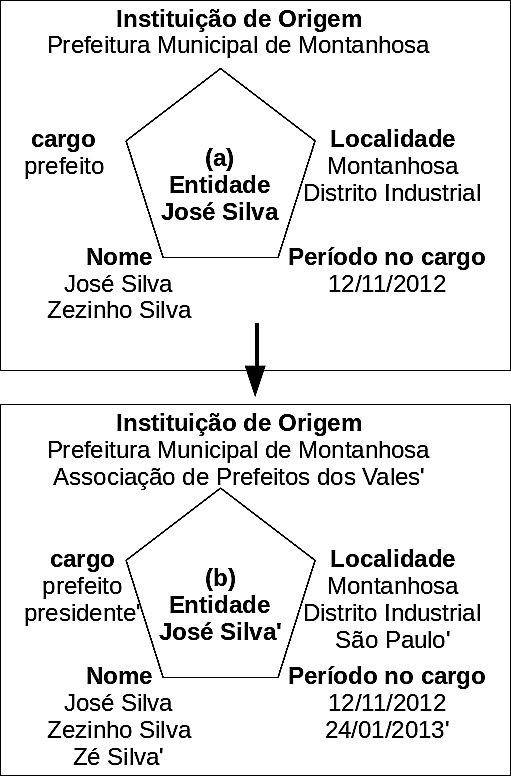
\includegraphics[width=.60\textwidth]{fig/facetasIndividuo.jpg}
%
%	\legend{Fonte: elaborada pelo autor}
%\end{figure}
%
%%\textbf{Exemplo didático da ata.}
%Um exemplo para o relacionamento entre entidades, facetas e termos, pode ser ilustrado por meio de uma ata de reunião, um típico documento de registro em instituições. O evento reunião teria acontecido em uma data, em um município e com participantes reconhecidos por nomes completos e suas respectivas instituições de origem. Um indivíduo denominado ``José Silva'' é uma entidade presente no documento, ilustrada na figura \ref{fig:facetasIndividuo} como um pentágono. Sua instituição de origem é a ``Prefeitura Municipal de Montanhosa'', onde está no cargo de ``prefeito''. \texttt{Nome}, \texttt{Instituição de origem}, \texttt{Cargo} e \texttt{Localidade} são facetas importantes para as entidades relacionadas a pessoas; e os termos ``José Silva'', ``Prefeitura Municipal de Montanhosa'' e ``prefeito'' estão associados às facetas na própria construção do texto da ata. O termo ``Montanhosa'' estaria associado à \texttt{Localidade} por dedução a partir da sua instituição de origem ou da localidade onde ocorreu a reunião. Facetas (em negrito) e seus respectivos termos constituem diferentes dimensões do pentágono (a) da figura \ref{fig:facetasIndividuo}.
%
%%\textbf{Motivação para o reconhecimento das facetas comuns.}
%Reconhecer esse conjunto de facetas comuns a maioria dos documentos é essencial para a organização automática da informação corporativa e para a interoperabilidade entre diferentes repositórios. Partindo do mesmo exemplo anterior, ao ser incluída uma nova faceta temporal \texttt{Período no cargo}, mesmo a data de início não tendo sido descrita na ata, sabe-se que na data da reunião ``José Silva'' era o prefeito em exercício. Assim, a \texttt{data de ocorrência} associada à reunião pode ser tomada como início do cargo de todas as entidades citadas no documento, inclusive da entidade ``José Silva''.
%
%%\textbf{Associação dinâmica entre facetas e focos/termos.}
%Essa associação entre localidades, datas, processos e entidades deve ser dinâmica e depende do reconhecimento de características espaciais, temporais, descritivas e lógicas. Nesse exemplo, a associação entre \texttt{data de ocorrência} da reunião e \texttt{período no cargo} de ``José Silva'' não é definitiva e vigora até que um novo documento evidencie uma data diferente para esta faceta, como é demonstrado na figura \ref{fig:facetasIndividuo}, em (b). Um documento de uma nova reunião ocorrida em São Paulo teria produzido as mudanças refletidas na entidade da figura \ref{fig:facetasIndividuo} (b), onde uma nova possibilidade de nome ocorre, a presidência de uma associação é registrada e o cargo de prefeito continua vigorando. A importância que esses novos termos assumem para cada faceta depende de muitas variáveis, como tempo, espaço, atores sociais envolvidos, a frequência e o uso dos novos e antigos termos nas mensagens que os documentos portam.
%
%%\textbf{Possibilidades para outros modelos de interação, como o ranking e a visualização.}
%A organização facetada da informação também torna mais flexíveis o \textit{ranking} e a visualização de resultados de busca. Na perspectiva de um usuário de informação, uma busca textual por ``negócios em montanhosa'' poderia muito bem retornar documentos de projetos em que ``José Silva'' seja citado mesmo que os termos ``Montanhosa'' ou ``Prefeitura Municipal de Montanhosa'' não estejam presentes. Adicionalmente, a própria desambiguação do termo montanhosa, uma cidade onde a organização possui unidade ou um adjetivo que pode pertencer a muitas entidades na coleção, é uma atividade necessária dentro do sistema de recuperação. Esse tipo de inferência espacial seria naturalmente realizado por um classificador humano experiente. Para uma busca ``negócios com prefeitura de montanhosa'', também seria natural que projetos recentes e antigos fossem recuperados, desde que incluam os nomes de ``José Silva'' ou de antigos prefeitos de Montanhosa, mesmo que os termos ``Prefeitura Municipal de Montanhosa'', ``prefeito'' ou ``Montanhosa'' não estejam explicitamente presentes no conteúdo do documento. Um buscador experiente poderia expandir a expressão de busca e incluir o nome dos vários prefeitos. Porém, uma organização de informação que inclua facetas espaciais, temporais, descritivas e lógicas também poderia subsidiar esses tipos de inferência, mas com a vantagem de considerar a temporalidade da informação, dos documentos e de cada prefeito-entidade indexado. Ou seja, não bastaria o modelo ser facetado para suportar buscas e recuperação de informação eficientes; o modelo precisa de facetas e tratamentos que realmente ajudem a evidenciar o contexto de entidades e documentos ao longo de todo seu ciclo de vida.
%
%
%
%
%
%
%%\textbf{Visão facetada do usuário.}
%Uma motivação tecnológica refere-se à visão facetada do usuário. Uma visão do esforço de busca do usuário informacional é a de que, ao invés de fornecer termos de interesse, o usuário normalmente fornece facetas de interesse. Por essa visão, caso o usuário de informação forneça um termo para espaço geográfico, como \emph{São Paulo}, seu interesse ultrapassa a existência do termo ou de uma notação para São Paulo, acrescentando à busca uma possibilidade de explorar a geografia do seu assunto de interesse. Na existência de um número como 1930 dado pelo usuário, se tem possivelmente uma faceta temporal pela qual a busca pode ser contextualizada e para qual até mesmo a terminologia do sistema de classificação precisa se adequar \cite{hong06,borges07,mir2ed}. Como exemplificado na seção anterior, se 1930 é um ano e São Paulo uma cidade ou estado, um documento com conteúdo que inclua \emph{adestramento} e \emph{mão de obra} refere-se provavelmente à capacitação dos funcionários das indústrias, o que requer um mapeamento de significado entre dois sistemas de classificação muito diferentes. 
%
%%\textbf{Diversidade e tamanho do conjunto de documentos impõem dificuldades.}
%Se explicar a intenção da busca em poucas palavras já parece difícil, mais difícil é a mesma intenção para espaços geográficos e janelas de tempo muito diferentes do espaço e do tempo da maioria dos documentos da coleção; e ainda mais difícil quando um componente de \textit{software} é o responsável por indexar e ``interpretar'' a necessidade de busca a partir de ideias e conceitos, recuperar documentos que possuem pouco mais que palavras e apresentar os resultados para o usuário de informação \cite{hong06}.
%
%%\textbf{Diversidade e tamanho do conjunto de documentos são ampliados quando o contexto é a Web.}
%A dificuldade é ainda maior no contexto de um sistema de recuperação de informação para documentos da \textit{World Wide Web} (WWW), ou um sistema de recuperação de informação de Internet. Na Internet estão documentos que versam sobre os assuntos mais diversos, em linguagem natural, sem metadados, nos mais diversos idiomas e linguagens especializadas \cite{hong06}. Neste caso, o sistema de classificação deve atender aos seguintes requisitos: 
%
%\begin{citacao}
%encontrar similaridade sem apenas encontrar padrões sem contexto; ser preciso e altamente descritivo; ser fácil de adicionar, apagar e atualizar classes e vocabulário sem a necessidade de reclassificar; deve suportar documentos digitais com uma informação que se expande continuamente \cite[p. 46, tradução nossa]{hong06}.
%\end{citacao}
%
%%\textbf{Web semântica e dados ligados como estratégias de enfrentamento tecnológico para a diversidade.}
%Para grupos específicos de documentos na Internet, ou para comunidades específicas de usuários, existe perspectiva de que as tecnologias de Web semântica e de dados ligados (\textit{Linked data}) farão maravilhas. Boa parte de seus trabalhos são baseados em metadados construídos voluntariamente por usuários, sem um compromisso adequado com o controle terminológico para a manutenção de longo prazo dos repositórios. 
%
%%\textbf{Facetas como recursos da navegação.}
%Facetas, ou os atributos que são chamados de facetas, normalmente servem principalmente ao propósito de navegar parte desses grandes repositórios \cite{oren06facetedRDF}. O reconhecimento de facetas facilita também a navegação nos resultados uma vez que há um refinamento possível para cada faceta, algo não facilmente alcançável em um sistema de recuperação de informação baseado em palavras do texto completo \cite{sacco2006,auer09linkedgeodata,docubrowse10,maculan2011,pontesLima2012}. Porém, ``sem um compromisso com vocabulários controlados, resta pouca esperança de que as tecnologias da Web semântica alcancem seu fim'' \cite[p. 269, tradução nossa]{labarre2010}, principalmente fora do escopo das coleções de documentos altamente estruturados como é o caso de bibliotecas de teses e dissertações, de patentes e de bancos de dados.
%
%%\textbf{Classificação facetada. Vantagens para documentos muito heterogêneos.}
%\citeonline[p. 47]{hong06} defende o uso de classificação facetada em sistemas de recuperação de informação muito heterogêneos:
%
%\begin{citacao}[english]
%faceted classification focuses on the essential and constant characteristics/facets, which is useful for micro-grained rapidly changing information repository. It can be used to create deeper and more complex knowledge structures by exploring variants of combination \cite[p. 47]{hong06}.
%\end{citacao} 
%
%%\textbf{Vantagens para a consulta.}
%A simplicidade dessa estrutura favorece os sistemas de recuperação de informação em que usuários devem buscar informação sobre entidades, espaços e tempos conhecidos \cite{toda08,entityCentric12}, especialmente no momento da consulta \cite{andrade06}. Este é o caso principalmente do contexto dos sistemas de recuperação de informação geográficos, em que espaço e tempo, duas facetas importantes em quase todo sistema de informação, são bem melhor estruturados e onde estão presentes alguns métodos de ordenação espaço-temporal.
%
%%\textbf{Vantagens para a ordenação.}
%Como exemplo, \citeonline{ehlen09} e \citeonline{toda08} descrevem aplicações para a ordenação baseada em múltiplas facetas, como a localização de documentos que pertençam à região de interesse do usuário, sendo que a relevância da faceta espacial é dada pela menor distância do ponto onde o usuário se encontra, o que é particularmente útil em serviços de localização e serviços móveis. A faceta temporal também é considerada em muitas aplicações em que novidades sobre um certo fenômeno, ao invés de relatos históricos, são preferíveis. É o caso de repositórios de notícias, serviços de monitoramento de catástrofe ou de trânsito. De fato, o interesse é por um método que consiga mensurar a importância do contexto geográfico, temporal ou temático em tempo de consulta \cite{andrade06} e responda com eficiência ao usuário de informação \cite{yuCai07,GarciaCumbreras09}.
%
%%\textbf{Vantagens para a manutenção.}
%Uma motivação metodológica refere-se à flexibilidade da classificação facetada. Como a classificação facetada é flexível e, portanto, adequada para modelar domínios em contínua expansão e mudança, mesmo os sistemas de classificação inicialmente implementados sem um sólido embasamento teórico podem ser beneficiados \cite{hong06,labarre2010}. Ou, em outras palavras, independentemente da qualidade da abordagem implementada pelos sistemas de recuperação de informação que se encontram na literatura, a teoria da análise facetada posta em prática no contexto desses sistemas e esses sistemas postos em avaliação sob a lente da teoria da análise facetada constitui um passo importante para a área.
%
%
%
%
%
%
%
%%\textbf{Link para próxima seção.}
%Na próxima seção são investigadas as principais pesquisas sobre avaliação de modelos de domínio e sobre avaliação de sistemas  de recuperação de informação, do desempenho dos processos de indexação e da recuperação de informação.
%
%
%\section{Avaliação de sistemas de recuperação de informação}
%
%%\textbf{Introdução.}
%Como a análise de domínio deve produzir um produto, um modelo de alto nível do domínio em estudo, após validado ele precisa ter sua utilidade avaliada. Também há muita diversidade de métricas de avaliação de utilidade desse tipo de instrumento, sendo que diferentes métricas refletem os objetivos do modelo, exatamente como acontece com a escolha dos métodos que são executados no processo de análise de domínio. Como o modelo resultante desta tese objetiva favorecer a atividade de recuperação de informação, sua avaliação se dá indiretamente, pela avaliação do desempenho da própria recuperação de informação.
%
%%\textbf{Coleções de referência.}
%A presença de uma coleção de referência favorece a comparação de sistemas de recuperação de informação e a definição de valores que sirvam como base de comparação. O contrário, quando experimentos são realizados em coleções privadas, a publicação de resultados se baseia muitas vezes em informação protegida, não disponível publicamente e muitas vezes sensível. Há muitas metodologias de avaliação de sistemas de recuperação de informação \cite{irEvaluation02,evaluationWithIncompleteInformation04,bucher05,sakai08ret,DBLP:conf/clef/2008}, algumas delas bem aceitas na indústria e na academia. Porém, há limitações para avaliação de sistemas corporativos pelas mesmas metodologias, dadas suas especificidades \cite{craswell05}.
%
%%\textbf{Coleção de referência Enterprise e as limitações para se constituir uma coleção.}
%Embora a trilha \textit{Enterprise} da \textit{Text Retrieval Conference} ofereça uma coleção de referência para sanar parte das limitações de avaliação; ao ser baseada apenas em documentos da \textit{Web} pública de uma empresa ela também se mostra insuficiente para avaliar a busca por recursos de informação reais \cite{bailey07}. Porém, a dificuldade de melhorar o \textit{corpus} de avaliação está na dificuldade de expor dados sensíveis de uma empresa, seus clientes, funcionários, fornecedores e suas estratégias de negócio. Mesmo uma empresa pública ou governo conta com informação sensível, protegida por lei, não sendo necessariamente um bom candidato a fornecedor de dados de avaliação. Por essa razão, muito do esforço de atingir os objetivos da trilha \textit{Enterprise}, que aconteceu até o ano de 2008, foi transferida para uma nova trilha, \textit{Entity Search} (ou, Busca por Entidades), que aconteceu até o ano de 2011, vislumbrando reconhecer entidades humanas e não-humanas e em diferentes escalas, das intranets de empresa à toda a Web \cite{balog08}.
%
%%\textbf{Avaliação em Fóruns de avaliação.}
%As técnicas e sistemas implementados têm sido confrontados com outros sistemas sob o mesmo prisma de avaliação, onde são encontradas várias metodologias. No entanto, os diferentes prismas e metodologias normalmente valorizam mais algumas fontes de evidências do que outros. É o caso da trilha \textit{GeoCLEF}, do \textit{Cross-Language Evaluation Forum} (CLEF), constituindo um \textit{framework} através do qual sistemas que utilizem linguagens europeias podem ser comparados sob os mesmos critérios e com a mesma massa de dados \cite{domenech07,cardoso08,anastacio09}, visando reconhecer evidências espaciais e linguísticas. Metodologia similar, porém específica para sistemas em língua portuguesa, é denominada Avaliação de Reconhecimento de Entidades Mencionadas (HAREM) \cite{harem07}.
%
%%\textbf{Avaliação através de Usuários de sistemas de recuperação de informação.}
%Outra estratégia de avaliação baseia-se na adoção direta dos usuários do sistema de recuperação de informação. É o caso do \textit{Open Directory Project} (ODP), onde são realizadas as mesmas atividades de avaliação e os resultados são comparados com aqueles anotados manualmente por voluntários \cite{amitay04}, e as metodologias de avaliação que empregam os próprios usuários do sistema como forma de avaliação mais criteriosa dos componentes de consulta e da qualidade percebida da resposta \cite{bucher05,yuCai07,pontes13}. Em todas as metodologias de avaliação são adotadas métricas muito próximas daquelas adotadas para sistemas convencionais, sendo que alguns trabalhos sugerem a necessidade de estabelecer metodologias mais adequadas para alguns tipos específicos de fontes de evidência e de coleções \cite{domenech07,sakai08ret}.
%
%%\textbf{Motivação para adotar duas coleções.}
%Um fórum que imponha o reconhecimento automático de diversos tipos de evidência, como espacial, temporal, social, linguístico e temático, por exemplo, não está disponível atualmente. Sua ausência, apesar de dificultar a tarefa de avaliação de sistemas de recuperação de informação, não representa o maior desafio de avaliação. O maior desafio continua a ser definir critérios formais de relevância, coleções de referência e métricas empíricas de desempenho adequados para diferentes atores sociais e contextos de uso. Por essa razão, esta pesquisa adota os resultados de \citeonline{bailey07} e \citeonline{balog08} como base de comparação, mas não pode dispensar uma avaliação complementar, com coleção privada e usuários reais, para garantir que os resultados realmente representem soluções de recuperação para situações mais próximas da realidade corporativa.
%
%%\textbf{A base metodológica para avaliação e as diferenças associadas.}
%Os procedimentos metodológicos para avaliação desta pesquisa sobre a coleção privada deve diferir pouco daqueles adotados por \citeonline{bailey07csiro}. A principal diferença é a perspectiva interpretativa adotada neste estudo; a importância dada à análise de domínio como componente formal da construção da coleção de referência e do modelo do domínio; o estabelecimento dos contextos de uso mais úteis para os usuários de informação; e o reconhecimento dos gêneros textuais e das linguagens adotadas por usuários e produtores de informação corporativa \cite{lykke2011domain}.
%
%
%
%
%%\section{Indexação}
%
%%?
%
%%linguística
%
%%temporal
%
%%geográfica
%
%
%%No entanto, entre os trabalhos encontrados, é senso comum que não há vantagem percebida em se usar técnicas geográficas ao invés das abordagens convencionais sobre o contexto geoespacial \citep{anastacio09,cardosoSantos08}, o que denota que muitos aperfeiçoamentos são ainda necessários em RIG. Identificados e descritos brevemente os principais trabalhos da área, é detalhado a seguir o projeto de pesquisa.
%
%
%
%
%
%%Considerações finais e trabalhos futuros
%
%%Esse capítulo empreendeu uma revisão de literatura sobre análise de domínio e organização da informação, comparando criticamente as abordagens intelectuais e automática que favorecem a classificação e indexação automáticas de coleções, usando ambientes corporativos como pano de fundo.
%
%
%
%
%
%
%
%
%
%
%
%
%%O acervo de informação, principalmente digital, de pessoas e empresas tem crescido significativamente pelas facilidades de produção, compartilhamento e armazenamento, este último parecendo quase não ocupar espaço físico pelos avanços tecnológicos.
%
%%No entanto, com esse crescimento, problemas associados à recuperação de informação têm surgido, sendo particularmente mais sérios quando a recuperação de informação é tarefa essencial para realizar trabalho e tomar decisões, algo que acontece em diversas áreas assim como em empresas.
%
%%São diversas as iniciativas que tentam minimizar os problemas de RI, especialmente da informação digital, mas iniciativas são mais efetivas quando baseadas em uma organização da informação adequada e compatível com a forma pela qual ocorre a organização do conhecimento.
%
%%Adicionalmente, com o ritmo acelerado da produção de informação, diversos desafios se impõem à classificação e indexação da informação por esforço intelectual, exigindo muitas vezes técnicas automáticas ou semiautomáticas de classificação e indexação com precisão e controle de erros altos. Por outro lado, o próprio desenvolvimento do conhecimento humano, a evolução das áreas de conhecimento e da linguagem.... criam obstáculos sérios para a eficiência destas técnicas automáticas, na convergência de esforços das ciências da informação, da computação, da linguística, da ciência cognitiva e outras.
%
%%Incluir justificativa para facetadas.
%
%%O estado da arte e da técnica da organização da informação visando a recuperação da informação, da informação digital especialmente, é a principal questão deste capítulo.
%
%%Além de objetivar mapear os principais trabalhos em organização da informação, este capítulo também se propõe a encontrar técnicas que favoreçam a classificação e indexação automáticas de coleções digitais, especialmente de documentos corporativos.
%
%%A organização organiza-se em X seções. Na primeira são tratadas as bases teóricas de classificação de informação, inclusive da organização multifacetada da informação. Na segunda, são apresentadas referências para técnicas de desambiguação e de indexação de tema, tempo e espaço, .... Finalmente, na terceira seção são discutidas as principais metodologias de avaliação da recuperação de informação.
%%bases teóricas de classificação
%%desambiguação de nomes de pessoas
%%desambiguação de nomes de empresas
%%desambiguação de sentido de palavras
%%desambiguação de tempo
%%desambiguação de espaço
%%indexação de pessoas
%%indexação de empresas
%%indexação de assunto (assunto? tema? termos?)
%%indexação de tempo
%%indexação de espaço
%%metodologias de avaliação
%%fóruns de avaliação
%
%
%%\section{Classificação de Informação}
%%Classificação
%
%%\section{Desambiguação e Indexação}
%%Desambiguação e Indexação
%
%%\section{Avaliação de Recuperação de Informação}
%%\label{avaliacao}
%
%%Avaliação de Recuperação de Informação
%
%
%%In despite of all these, regretfully, we still tend to put all bets on technology every time new technology appears. In answering the question of why it is so hard to find information on the Web, and why search engines aren't more helpful?, Rosenfeld replied that one reason for this confusion is that it's really hard to express our information needs in words, much less translate those words into a query language understood by a dumb piece of software (that is, search engines). Another reason is that it's really hard to index the ideas and concepts that are stored in text in a way that this dumb software can understand (and therefore find). So when we do a search, we're asking something much dumber than we are to do something we find hard to do ourselves'' [Morville, 2002]
%
%%\citep{hong06}
%
%%As formas pelas quais as pessoas buscam na Web e na empresa tendem a ser semelhantes. Por isso, muitos dos problemas percebidos pelos usuários e relacionados à consulta e ao \textit{ranking} são comuns.
%
%
%
%
%
%
%
%
%
%%Definições
%%Indexação
%%Indexação é o processo intelectual que envolve atividades cognitivas na compreensão do texto e a composição da representação do documento. E, por ser uma atividade intelectual, pode se beneficiar particularmente de teorias e métodos da Psicologia Cognitiva e da Teoria de Soluções de Problemas (David et alii, 1995, p.49). Wellish (1995)**, citado por Jacob & Shaw (1998, p.159), descreve indexação como o ato de indicar ou apontar o conteúdo intelectual de uma coleção. Esta definição mascara a natureza cognitiva do processo de indexação, por enfatizar o produto físico do processo, e não a análise de conteúdo.
%%Conceito
%%
%%Termo
%%
%
%
%
%%A principal metodologia de projeto e implementação de um sistema de recuperação de informação geográfica (RIG) baseia-se em um sistema de RI convencional, com os mesmos componentes, onde são implementadas as técnicas de tratamento da informação geográfica \cite{anastacio09, cardosoSantos08}. Com isso, os componentes incluem os métodos de coleta de documentos, de reconhecimento de entidades ou \textit{geoparsing} e de identificação e desambiguação dessas entidades ou geocodificação. A tarefa de indexação, do conteúdo e das referências geográficas reconhecidas, também faz-se necessária para manter o sistema em condições de fornecer respostas precisas e eficientes, enquanto que a interface com o usuário e o componente de classificação e ordenação desempenham papel importante para atender seu usuário.
%
%
%
%%\section{Recuperação de informação corporativa}
%
%%Enterprise Information Retrieval
%
%%Principais diferenças. Cabe aqui ou ao longo da revisão de literatura?
%
%%Estudos sobre o custo de tempo necessário para realizar pesquisas na empresa
%
%%Pesquisa como parte de tarefas próprias da rotina empresarial. Exemplos de tarefas.
%
%%A eficiência para o usuário de um sistema de recuperação de informação se reflete em custos menores para a organização, no contexto de EIR, que garante continuidade de negócios, escalabilidade, privacidade.
%
%%Arquitetura de um SRI corporativa. Cada componente da arquitetura refere-se a uma fase a ser apresentada a seguir.
%
%
%
%
%
%
%
%
%%\section{Coleta}
%
%%Crawler
%
%%Fontes internas e externas.
%
%%Preservação do documento original apresenta riscos para segurança e nem sempre é possível.
%
%%No caso de federação, nem sempre é possível ter acesso aos documentos. Só é possível encaminhar pesquisas e mesclar os resultados com o resultado final ao usuário.
%
%%Quando há muitas réplicas do mesmo documento, um problema caro de resolver é exposto, com risco para segurança em caso de informação sensível ou dificuldades de armazenamento ou processamento para identificação da réplica.
%
%%Aplicação de hash para controle de alteração. Versões do documento. Nova coleta do documento. Problemas das réplicas identicas ou levemente modificadas.
%
%
%
%%Faltam detalhes do coletor/crawler
%
%%Textos, imagens, sons, desenhos
%
%%Diferentes formatos de arquivos e codificação de dados
%
%%Presença de dados em arquivos, bancos de dados distribuídos em servidores e clientes por toda a empresa e fora dela
%
%%Compactação, criptografia
%
%%Acessibilidade limitada à informação por dificuldades de permissões, conectividade, baixa qualidade de metadados
%
%
%%\section{Parsing e reconhecimento de entidades}
%
%
%%Os documentos, materializados em arquivos, normalmente contam com metadados em seu formato original. Porém, tais metadados não estão sempre disponíveis. Frequentemente são imprecisos, estáticos e desatualizados.
%
%%Especialmente em um contexto de pesquisa multifacetada, o reconhecimento de entidades assume particular importância para a eficiência do SRI como um todo, e para a organização da informação, em particular.
%
%%Processar o máximo de texto dos documentos, porém nem todo documento tem seu texto disponível para processamento.
%
%%Documentos podem estar compactados, criptografados, protegidos contra extração de texto, codificados em formato proprietário, corrompidos, etc.
%
%%Outra classe de problema trata do reconhecimento de entidades/facetas por padrão de texto, proximidade de um termo em relação a outros, localização no documento (início, meio, fim) e através de outras fontes de evidência para adequada desambiguação e correta indexação.
%
%
%
%
%
%
%
%%\section{Indexação}
%
%%Indexar o máximo de fontes de evidência de relevância leva a aumentar o número de facetas sobre as quais documentos e informação são classificados.
%
%%Algumas fontes de evidência podem ser:
%%local físico
%%geográfico
%%tipo de arquivo/formato
%%nome do arquivo
%%tipo do documento e outras informações mais.
%
%%Também são úteis metadados do administrador, do usuário, texto completo, data de produção, volumes de réplicas, referências a nomes de entidades/facetas, idioma, cliques sobre o documento ou frequência de uso do documento pelo grupo, pelo usuário, pela empresa.
%
%%Os principais problemas são: como tratar a diversidade de tipos, a ausência de atributos de alguns com a presença de outros, o custo da estrutura de dados e do acesso a tantas facetas, a importância dos arquivos sobre outros para os quais não há permissão de acesso, como indexar sem que a recomposição de arquivos sensíveis seja possível, como identificar réplicas e versões com menor custo, a identificação do idioma e como priorizar idiomas, como indexar múltiplos idiomas, qual estrutura adotar para cada faceta, como indexar perfis de usuários e se é necessário. Como um perfil de usuário pode parametrizar interesse ou prioridade de umas facetas sobre outras.
%
%%Atualização de índice
%
%%Múltiplas facetas requerem estrutura ou estruturas próprias?
%
%%Um índice por faceta? Ou um para todo o conjunto?
%
%%Um índice por repositório ou um índice para todo o conjunto?
%
%
%
%%\section{Consulta}
%
%%A forma através da qual o usuário interage com o sistema pode impactar na qualidade dos resultados e do sistema como um todo. Para isso, um componente essencial é a interface de consulta, onde o usuário fornece seus interesses, temáticos ou espaciais. Nesse local, duas abordagens possíveis são a separação da entrada de tema e espaço \citep{yuCai07} ou a reunião de ambos no mesmo ponto de entrada, sendo necessários o \textit{geoparsing} e a geocodificação, assim como ocorrem no conteúdo dos documentos, também no texto da entrada. Trabalhos relacionados a identificação geoespacial na consulta têm sido realizados também por \citet{gan08}.
%
%%influência da IU na experiência e satisfação do usuário.
%
%%Identificação de termos e facetas de interesse do usuário. Atributos do usuário como quem, onde, quando, como, porquê.
%
%%Como fazer um parsing adequado para cada usuário.
%
%%Busca dinâmica facetada \citep{pontesLima2012}.
%
%%Como os resultados devem ser visualizados? Colunas, ícones, visualizações. Não é bem para consulta ou consulta interativa, mas está dentro de IU.
%
%%Consulta em contexto: local, momento, quem, porquê, como, ...
%
%%Qual o conjunto de repositórios mais relevante para o usuário naquele contexto de busca? Este problema se junta ao processamento da consulta.
%
%%\section{Processamento de consulta}
%
%%Qual o conjunto de repositórios mais relevante para o usuário naquele contexto de busca? Este problema se junta ao processamento da consulta.
%
%%Federação ou centralização de metadados.
%
%%Segurança do sistema e dos dados. Acesso remoto. Acesso interno.
%
%%Estatísticas e logs de acesso. Eficiência computacional para acesso às estruturas de dados, localização de termos, seleção e ordenação de registros.
%
%%Processamento distribuído
%
%%Controle de acesso - segurança - direito
%
%%Information Filtering
%
%%Profiles
%
%
%
%
%%A forma através da qual o usuário interage com o sistema pode impactar na qualidade dos resultados e do sistema como um todo. Para isso, um componente essencial é a interface de consulta, onde o usuário fornece seus interesses, temáticos ou espaciais. Nesse local, duas abordagens possíveis são a separação da entrada de tema e espaço \citep{yuCai07} ou a reunião de ambos no mesmo ponto de entrada, sendo necessários o \textit{geoparsing} e a geocodificação, assim como ocorrem no conteúdo dos documentos, também no texto da entrada. Trabalhos relacionados a identificação geoespacial na consulta têm sido realizados também por \citet{gan08}.
%
%
%
%%\section{Ranking ou Ordenação}
%
%%problemas com TFIDF
%
%%\citep{akritidis11} para ranking
%
%
%%Quais propostas existem?
%
%%Colunas para diferentes tipos de dados, com ranking diferente
%
%%Combinação de rankings
%
%%Pesos
%
%%Criação de profiles
%
%%A partir do reconhecimento de facetas, o ranking pode ser adaptativo?
%
%%Ranking de relevância a partir de facetas organizadas em estruturas de dados diferentes, ao invés de métricas baseadas na frequência da ocorrência de termos.
%
%%Outro problema relevante é a ordenação ou \textit{ranking} de documentos para a construção da resposta ao usuário. Na área de RIG, dada uma entrada do usuário, é necessário ordenar os documentos que eventualmente atendam ao seu interesse, combinando as variáveis temáticas e espaciais. Porém, tal ordenação mostra-se complexa uma vez que é difícil assinalar qual faceta é a mais importante ao usuário, se o tema de interesse ou a região de interesse. É provável que por este problema os sistemas geográficos ainda não apresentem ganhos significativos de precisão nas consultas se comparados aos sistemas convencionais.
%
%%A maioria dos trabalhos projeta um sistema que usa dois índices para o \textit{ranking} do resultado de consulta, um baseado na relevância do texto ou conteúdo do documento e outro baseado no contexto espacial, havendo diferenças substanciais na parte geográfica entre os trabalhos. A própria tarefa de indexação de cada documento normalmente é realizada em separado, sendo que cada documento é georreferenciado e alocado no espaço de coordenadas geográficas ao mesmo tempo em que é indexado por seus termos no espaço vetorial \citep{yuCai07}. 
%
%%\Citet{li06} implementam a ordenação geográfica por meio de uma matriz pela qual a superfície da Terra é dividida. \citet{martins10} usam métodos de aprendizado de máquina para a criação do \textit{ranking} temático e geográfico em uma única função de ordenação por relevância, baseada na estratégia \textit{Learning to Rank}. \citet{ehlen09} e \citet{toda08} focam outras aplicações para a ordenação, como a localização de documentos que pertençam à região de interesse do usuário, sendo que a relevância do espaço geográfico é dada pela menor distância do ponto onde o usuário se encontra, o que é particularmente útil em serviços de localização e serviços móveis. De fato, o interesse é por um método que consiga mensurar a importância do contexto geográfico ou temático em tempo de consulta \citep{andrade06} e responda com eficiência ao usuário \citep{GarciaCumbreras09, yuCai07}.
%
%
%
%
%
%%\section{Atualização da coleção}
%
%%Arquivos são atualizados e sua relevância pode mudar em função de tais atualizações.
%
%%Eficiência da coleta de arquivos para verificação de atualização.
%
%%Da reindexação de arquivos atualizados. Da exclusão de arquivos do índice. Da inclusão de novos arquivos. Eficiência tanto para armazenamento quanto para processamento de indexação, de consultas e de verificação de alteração.
%
%
%
%
%
%
%
%
%%Métricas?
%
%%EIR contam com repositório de avaliação? TREC?
%
%%Quais outras propostas existem para avaliação? Como discutem a eficiência delas?
%
%
%
%
%
%
%
%
%%\section{Recuperação de informação multifacetada}
%
%%O título está ok?
%
%%Quais facetas exemplificar?
%
%%Em um SRI geral, para Web, e Enterprise?
%
%%Os sistemas tendem a ser estatísticos, algo que provoca insatisfação ao usuário.
%
%%Um passo adiante é necessário para aumentar a satisfação do usuário, pelo melhoria de métricas comuns como precisão e revocação, mas também pela redução do custo de tempo para o uso de SRI, algo particularmente útil no contexto de EIR.
%
%%Custo de tempo não significa um sistema simplesmente mais rápido, mas um processo de busca por informação que encerra no menor tempo possível, entre seu início e a localização de toda a informação necessária para se realizar uma tarefa.
%
%%Quais atributos podem ser usados da coleta para ajudar no reconhecimento de facetas? E no parsing? E como o índice deve ser implementado?
%
%%Quais alterações devem ser realizadas na busca (IU)? Quais as implicações deste modelo para o processamento? E para a atualização?
%
%%docubrowse \cite{docubrowse10}
%
%
%
%
%
%
